\chapter{Implementación}

La implementación del software se ha dividido en hitos. Estos han sido definidos en GitHub
y cada uno de ellos contiene un grupo de \textit{issues} que se corresponden con las distintas
mejoras que se han ido incorporando al software a lo largo de su desarrollo.\\

\section{Primeros planteamientos para el proyecto}

\subsection{Proyecto como aplicación final}

Los primeros pasos para afrontar este proyecto se hicieron proponiendo crear dos
aplicaciones reproductoras de audio, una para Android y otra para Linux. Ambas
tendrían acceso a una misma biblioteca compartida de archivos MP3, la cual
estaría en red, por lo que ambos reproductores tendrían conocimiento y acceso a
la misma colección de audio. En dicha biblioteca todos los elementos estaría
asociados a un identificador, por lo que cuando el móvil y el altavoz se
comunicasen a través del NFC, se transferiría el identificador del archivo de la
reproducción actual, además del segundo actual. De esta forma el altavoz sabría
que elemento de la biblioteca reproducir y en que segundo comenzar.

El problema de esta solución era que la biblioteca dependía del usuario final,
por lo que conllevaba andar añadiendo canciones y podcast manualmente, como si
de 2008 se tratase... Por tanto, generaba más problemas de los que solucionaba,
por lo que se decidió darle al proyecto un enfoque como servicio en lugar una
aplicación para un usuario final.

De esta manera, el proyecto como servicio sería integrado por otras aplicaciones
de reproducción, dejando el tema de proveer el contenido a cargo de las mismas.

\subsection{Proyecto como servicio - Google Cast}

Al enfocarlo como servicio se propuso emplear algún protocolo amplio y conocido
como es \emph{Google Cast} \cite{google-cast}, de modo que el receptor de audio
fuese un servidor de \emph{Google Cast}, y el servicio en \emph{Android}
estuviese a la espera de una interacción NFC para conectarse mediante
\emph{Cast} al servidor con el que se hubiese comunicado. 

El problema que hubo con este planteamiento y por lo que también se descartó es
que Google no permite que dispositivos ``no genuinos'' sean usados como
servidores de \emph{Google Cast}. Esto significa que únicamente se permite dotar
de servidor \emph{Cast} a los dispositivos licenciados por \emph{Google} como
pueden ser los \emph{Google Chromecast, Google Home, Google Nest, etc}. Por lo
que hubo que desechar ese protocolo de transmisión y buscar otra alternativa
libre.

\subsection{Proyecto como servicio - HLS/WebRTC/RTSP}

Al desechar el uso de \emph{Google Cast} hubo que bajar un nivel de abstracción
para buscar alternativas libres y desarrollar un \emph{Google Cast} propio que
permitiese enviar el audio a un servidor. Tras el estudio de las \emph{API} de
\emph{Android} se optó por emplear la \emph{API} existente en \emph{Android 10
(SDK29)} llamada \emph{AudioPlaybackCapture} \cite{api-audio-capture}, la cual
permite capturar el audio interno de \emph{Android}, para posteriormente
procesarlo, grabarlo, o trabajar libremente con él. Por lo que el nuevo enfoque
sería enviarlo a través de cualquier protocolo de streaming como puede ser \emph{HLS,
WebRTC o RTSP} tras capturarlo con la mencionada \emph{API}.


\section{Selección del lenguaje de programación}

Dentro del proyecto se ven involucrados más de un dispositivo, ya que coexisten
dispositivo móvil y receptor. Ambos podrían llegar a programarse usando el mismo
lenguaje, lo cual sería ventajoso, puesto que, se unificaría el \emph{toolchain} e
incluso se podría ahorrar código. Pero dado que existen requisitos o
dependencias más prioritarias (las cuales serán detalladas en los requisitos de
búsqueda y selección), la elección se dejará a juicio del proceso de selección.

\subsection{Dispositivo móvil}

En este aspecto no tenemos mucho donde elegir. Si hablamos de dispositivos
móviles estamos hablando de \emph{Android} e \emph{iOS}. Y puesto que ya
descartamos \emph{iOS} en la introducción del problema, por ser un sistema
operativo más cerrado y buscar centrarnos en un sistema operativo abierto, el
sistema operativo móvil sobre el que se centrará el proyecto será \emph{Android}.

Si queremos programar en \emph{Android} primero debemos decidir si queremos hacer una
aplicación nativa, híbrida o generada \cite{nativo-hibrido-generado}. Las
aplicaciones nativas se programan en lenguajes con soporte nativo por el sistema
operativo, por lo que tienen un aspecto más similar al propio sistema operativo,
y un mejor rendimiento, sin embargo, requieren de más esfuerzo de desarrollo. Las
aplicaciones híbridas son aplicaciones web que se ejecutan en un navegador web
simulando ser una aplicación nativa, por lo que la interfaz no suele tener un
aspecto tan uniforme al sistema y el rendimiento suele ser notablemente
inferior. Y las generadas son aplicaciones que se programan en un lenguaje no
nativo, pero que mediante un \emph{framework} son traducidas a lenguajes nativos, sin
embargo, al depender de traducción el rendimiento no llega a ser el mismo que el
de una aplicación nativa.

A la hora de elegir qué usar para este proyecto entre los tres tipos de
aplicaciones mencionados, la interfaz gráfica no es algo a tener en cuenta, ya
que, no vamos a hacer una aplicación como tal, sino un servicio para que otras
aplicaciones implementen. Sin embargo, sí que tenemos que tener en cuenta el
rendimiento así como el acceso y manejo con el sistema operativo o con
componentes hardware de más bajo nivel, como es el \emph{NFC}. Para estos casos las
aplicaciones nativas son una mejor elección, ya que, al existir menos capas entre
la aplicación y el sistema operativo, obtienen un mejor rendimiento, y facilitan
la comunicación con componentes hardware de bajo nivel. Lo cual nos lleva a
optar por una aplicación nativa.

Para programar una aplicación nativa existen varios lenguajes que lo permiten
\cite{lenguajes-nativos}, sin embargo, dado que vamos a requerir de comunicación
con elementos hardware como es el lector \emph{NFC}, vamos a optar por lenguajes
que tengan una documentación extensa y detallada en cuanto a desarrollo móvil y
comunicación con \emph{Android}, reduciendo estos lenguajes nativos a \emph{Java} y
\emph{Kotlin}, puesto que, son para los que existe más bibliografía y ejemplos
relacionados con este sistema operativo móvil.

Finalmente, para optar por uno u otro, \emph{Google} lo tiene claro, ya que desde 2019
están enfocados en \emph{Kotlin} y buscan que sea el principal lenguaje de \emph{Android}
\cite{prioridad-kotlin}. De hecho como ellos mismos explicaron, desde 2019 cada
vez que desarrollan una \emph{API} o contenido nuevo lo hacen teniendo en mente
el uso con \emph{Kotlin}, por lo que este lenguaje será el más indicado si lo que
pretendemos es usar alguna \emph{API} que se comunique con el \emph{NFC} del
sistema \emph{Android}.

Así que, teniendo todo esto en cuenta, el lenguaje utilizado para el
dispositivo móvil será \textbf{\emph{Kotlin}}

\subsection{Dispositivo receptor: módulo NFC}

Este dispositivo utilizará \emph{Linux}, ya que es el sistema operativo que está
presente en casi la totalidad de placas de desarrollo y mini PC que lo cual
facilitará enormemente el desarrollo. 

\subsubsection{Criterios de búsqueda}

Dado que correr \emph{Linux} no es algo limitante a la hora de elegir lenguaje de
programación, el principal factor que fijará el criterio de búsqueda es la
compatibilidad con librerías NFC actualizadas.

\begin{itemize}
    \item Debe de ser compatible con librerías NFC.
    \item Debe ser un lenguaje tocado previamente en alguno de los años del grado.
\end{itemize}

\subsubsection{Criterios de selección}

Las propuestas encontradas bajo los criterios de búsqueda serán evaluadas bajo
los siguientes criterios de selección:

\begin{itemize}
    \item La librería debe estar mantenida o recibir actualizaciones cada poco tiempo.
    \item Debe de tener documentación extensa en la que se valorarán los ejemplos ya hechos.
    \item La instalación de la misma debe de ser lo más simple posible.
    \item Se valorará muy positivamente la facilidad o simplicidad del lenguaje a la hora de manejar los datos a enviar o recibir con el NFC.
\end{itemize}

\subsubsection{Opciones encontradas según los criterios de búsqueda establecidos}

\begin{itemize}
    \item Java: \href{https://github.com/grundid/nfctools}{nfctools}. Si bien al
    hablar de Java esperaba que existiese una gran cantidad de librerías, no han
    sido tantas las encontradas. Siendo la mayoría librerías comerciales para
    lectores NFC concretos.
    \item Python: \href{https://github.com/nfcpy/nfcpy}{nfcpy}. Al igual que con
    Java, la búsqueda ha devuelto menos librerías de las esperadas. Aunque en
    este caso casi todas las entradas y proyectos existentes con NFC en Python
    apuntaban a esta librería.
    \item C: \href{https://github.com/nfc-tools/libnfc}{libnfc}. 
    \item C++: \href{https://github.com/liblogicalaccess/liblogicalaccess}{LibLogicalAccess}.
\end{itemize}

\subsubsection{Proceso de selección y estudio}

\subsubsection{Java: nfctools}

\begin{todolist}
    \item El repositorio de \href{https://github.com/grundid/nfctools}{GitHub}
    no ha recibido actualización desde 2014. Si bien algún colaborador ha
    seguido trabajando en su propia rama del proyecto algún tiempo, los cambios
    ni siquiera han sido fusionados con \emph{master} e incluso esa rama más
    actualizada lleva 3 años sin un \emph{commit}. Por lo que este requisito no lo
    cumple dicha librería, y, por tanto, tampoco Java.
    \item Esta librería no tiene documentación más que el
    \href{https://github.com/grundid/nfctools/blob/master/README}{README de
    GitHub} y la \href{https://www.grundid.de/nfc/index.html}{web del proyecto},
    la cual hace más de portal inicial que de documentación. Por lo que no
    cumple este requisito.
    \item Al no tener documentación hace que el proceso de instalación requiera
    de intentos a ciegas, investigación y avances según prueba y error. Por lo
    que no cumple este requisito.
    \item[\xcmark] Java es un lenguaje con el que se puede trabajar y manejar
    los datos de forma medianamente fácil, ya que dispone de clases hechas que
    automatizan y facilitan parte del proceso. Aunque igualmente si se compara
    con otros lenguajes habrá alternativas que simplifiquen aún más el proceso.
    Sin embargo, considero este requisito como válido.
\end{todolist}

\subsubsection{Python: nfcpy}

\begin{todolist}
    \item [\xcmark] El último \emph{commit} en el repositorio de
    \href{https://github.com/nfcpy/nfcpy}{GitHub} fue en marzo de 2022 cuando
    lanzó el último \emph{release}. Mientras que la última actividad del principal
    contribuidor de la organización que lleva el repositorio fue a finales de
    agosto contestando issues; por lo que podemos decir que aunque no de manera
    continuada o diaria, la librería sigue recibiendo soporte y está activa, por
    lo que cumple este requisito.
    \item [\xcmark] Posee
    \href{https://nfcpy.readthedocs.io/en/latest/index.html}{readthedocs} en
    donde se detallan los primeros pasos, instalación, ejemplos, etc. Es
    bastante completa y concisa por lo que también satisface con creces este
    requisito.
    \item [\xcmark] Para instalarlo basta con emplear pip, ya que está publicado en
    \href{https://pypi.org/project/nfcpy/}{PyPi}. Por lo que se instala de una
    forma rápida y sencilla.
    \item[\xcmark] Python es uno de los lenguajes más simples y sencillos de
    usar, especialmente como se está viendo últimamente para el manejo de datos,
    por lo que este requisito lo cumple de manera sobrada.
\end{todolist}

\subsubsection{C: libnfc}

\begin{todolist}
    \item [\xcmark] El último \emph{commit} del repositorio de
    \href{https://github.com/nfc-tools/libnfc}{GitHub} fue en febrero de 2023,
    por lo que podríamos decir que si mantiene el soporte, sin embargo,
    revisando los \emph{issues} y los \emph{pull request} están en su mayoría
    desatendidos desde hace años. Y de hecho los \emph{commits} de los últimos años son
    simplemente de fusionar algunos PR aceptados, por lo que da la sensación que
    el soporte que recibe es el de comprobar cada ciertos meses los \emph{pull
    request} activos y aprobarlos si son cambios que no requieren mucha
    intervención. Sin embargo, aún sabiendo esto, interpretaré como que recibe
    soporte, ya que en cierto modo es así.
    \item Posee cierta documentación muy básica en el README del repositorio, y
    adicionalmente tienen \href{nfc-tools.org}{una web} en la que se supone que
    tienen una comunidad, una wiki detallada, etc. Pero esta web no responde en
    el momento de hacer el estudio, por lo que se entiende que la web ha sido
    abandonada, por tanto, no cumple este requisito.
    \item Para instalar la librería primero hay que clonar el repositorio,
    ejecutar el \emph{script} de configuración y una vez generados los archivos
    de configuración, compilar con \emph{make}, para después finalmente ejecutar otro
    \emph{make install}. Una vez completado el \emph{makefile} hay que copiar los binarios
    resultantes a cierta ruta y configurar el \emph{path}. Aunque son unos pasos
    no muy complicados que cualquier estudiante del grado podría superar, no es
    un proceso rápido o sencillo si lo comparamos con el de la librería de
    Python la cual se instalaba automáticamente con pip. Por tanto, considero que
    no supera este requisito.
    \item C no es un lenguaje especialmente simple a la hora de tratar con
    datos, pues no dispone de una STL como es el caso de C++ en el que se
    simplifique el trabajo con vectores etc. Habría que hacerlo manualmente con
    malloc, calloc, free, etc. Por lo que se aleja mucho de la simplicidad o
    facilidad para el manejo. Debido a esto, no supera el requisito.
\end{todolist}

\subsubsection{C++: LibLogicalAccess}

\begin{todolist}
    \item [\xcmark] El último \emph{commit} del repositorio de
    \href{https://github.com/liblogicalaccess/liblogicalaccess}{GitHub} fue en
    marzo de 2023, y los \emph{issues} y \emph{pull request} se mantienen todos
    atendidos, por lo que denota que se mantiene activo y con soporte del
    desarrollador. Por tanto, cumple este requisito.
    \item [\xcmark] Utiliza la wiki de GitHub a modo de documentación, teniendo
    documentado el proceso de instalación y algunos ejemplos en hardware
    concreto. Además, posee una \href{https://liblogicalaccess.com/}{web oficial}
    en la que tienen publicado el Doxygen. Podemos decir que cumple dicho requisito,
    aunque comparando con algunas otras alternativas vistas, no es la más
    completa.
    \item Para instalar la librería hay que utilizar un software llamado
    \href{https://conan.io/}{conan}, el cual es un gestor de paquetes para C y
    C++ tras clonar y compilar el repositorio con conan. Adicionalmente, este
    software se instala a través de pip, por lo que habría que instalar también
    pip, ya que con una instalación de gcc no se instala. Por tanto, no considero
    que sea una instalación necesariamente simple, por lo que no cumple este
    requisito.
    \item [\xcmark] A pesar de que C++ tiene la STL la cual simplifica mucho el manejo de
    datos con las clases ya hechas y la automatización de la memoria dinámica
    que se hace dentro de la misma, el manejo de datos no es la tarea más simple
    dentro de C++. Sin embargo, aunque sea por los pelos o ``cogido con pinzas'',
    daré como cumplido este requisito.
\end{todolist}

\subsubsection{Conclusión}

Tras valorar mediante los criterios de selección los lenguajes principales
encontrados según los criterios de búsqueda, podemos ver que el lenguaje que
satisface todos los criterios es \textbf{Python con la librería nfcpy}. Por lo que este
será el lenguaje empleado para el módulo NFC en la parte del receptor.

\subsection{Dispositivo receptor: módulo audio streaming} \label{seleccion-streaming-receptor}

Este dispositivo es el mismo que el que ejecutará el módulo de NFC, sin embargo,
para reproducir el audio en streaming se tendrán unos requisitos diferentes que
para el estudio anterior, por lo que será necesario un proceso de selección
nuevo con los nuevos criterios.

\subsubsection{Criterios de búsqueda}

Para capturar y enviar el audio desde la parte de Android se emplean bibliotecas
de Java. Por lo que el lenguaje que se emplee para el audio en streaming debería
ser compatible con esas bibliotecas, ya que de esta forma se reduciría bastante
el tiempo de programación pues con los conceptos y funciones aprendidos para la
parte del dispositivo Android, cubriríamos también los del receptor. A su vez al
utilizar las mismas bibliotecas se reducirían los posibles errores o
incompatibilidades. Por lo que los criterios de búsqueda serán:

\begin{itemize}
    \item Debe de tener compatibilidad nativa con las mismas librerías empleadas
    en la parte del dispositivo Android.
    \item No se tendrán en cuenta las variantes de otros lenguajes de
    programación que traducen en tiempo real el código a Java (Jython, JGo,
    JRuby, etc.)
\end{itemize}

\subsubsection{Criterios de selección}

Las propuestas encontradas bajo los criterios de búsqueda serán evaluadas bajo
los siguientes criterios de selección:

\begin{itemize}
    \item La instalación del lenguaje en modo \emph{headless} debe ser lo más simple posible.
    \item La ejecución de código debe de ser lo más simple posible.
    \item Se valorará positivamente el haberse estudiado en algún momento a lo largo del grado.
\end{itemize}

\subsubsection{Opciones encontradas según los criterios de búsqueda establecidos}

\begin{itemize}
    \item \href{https://www.java.com/es/}{Java}.
    \item \href{https://kotlinlang.org/}{Kotlin}.
    \item \href{https://groovy-lang.org/}{Groovy}
    \item \href{https://www.scala-lang.org/}{Scala}
\end{itemize}

Todos estos lenguajes soportan nativamente las bibliotecas de Java, ya que todos
se ejecutan sobre la JVM.

\subsubsection{Proceso de selección y estudio}

\subsubsection{Java}

\begin{todolist}
    \item[\xcmark] Java es un lenguaje muy extendido y conocido, así como
    antiguo, por lo que al llevar tanto tiempo usándose y por
    \href{https://www.stackscale.com/es/blog/lenguajes-programacion-mas-populares/}{una
    cantidad tan grande de usuarios} ha hecho que esté disponible para su
    descarga e instalación en casi la totalidad de repositorios de cada
    distribución (apt, yum, etc.). Por lo que el proceso de descarga, instalación
    y configuración del path queda simplificado a un simple ``apt install
    default-jre'' en el cual incluso se puede especificar fácilmente si se
    necesita alguna versión en particular. Satisfaciendo de forma sobrada este
    requisito.
    \item[\xcmark] Para la ejecución de código en Java gracias a la JVM basta
    con ejecutar el comando ``java'' seguido del archivo con el código, sin
    necesidad de añadir flags ni generar binarios para su posterior ejecución
    manual. Por lo que cumple este requisito.
    \item[\xcmark] Java es un lenguaje bastante utilizado a lo largo del grado,
    en asignaturas como PDOO (Programación y Diseño Orientado a Objetos), FR
    (Fundamentos de Redes)y SM (Sistemas Multimedia); por lo que la curva
    inicial de aprendizaje ya ha sido sobrepasada y no es un lenguaje en el que
    se tenga que empezar de 0.
\end{todolist}

\subsubsection{Kotlin}

\begin{todolist}
    \item Para instalar Kotlin, dado que es un lenguaje mucho más moderno que
    Java, aún no ha sido añadido a los repositorios que vienen por defecto en
    las distribuciones Linux. Por lo que para instalarlo habrá que descargar los
    binarios pre compilados accesibles oficialmente desde GitHub según la
    versión específica a emplear o instalarlo desde un repositorio de terceros
    llamado \emph{SDKMAN} el cual si trae el paquete de Kotlin en su catálogo, y
    permite especificar la versión deseada, pero que para usarlo es necesario
    instalarlo previamente también. Por lo que si bien estos pasos no son
    complicados, al ponerlo en comparación con Java, este queda en peor lugar,
    por lo que no cumple este requisito.
    \item A pesar de que al igual que Java, utiliza la JVM para funcionar, a la hora
    de compilar y ejecutar código
    \href{https://stackoverflow.com/a/69030563}{vemos} que el proceso puede
    variar dependiendo de si es código nativo de Kotlin o si no lo es. Por lo
    que hay que tener en cuenta si añadir el \emph{runtime} para que se pueda ejecutar
    o no, entre otros flags, para generar el ejecutable que posteriormente
    podemos ejecutar. Por lo que al igual que en el requisito de antes, aunque
    no es un proceso complicado y que de hecho está bastante simplificado, si lo
    comparamos con el otro lenguaje analizado, el proceso de Java sigue teniendo
    un proceso más simple para ejecutar el código. Por lo que Kotlin tampoco
    cumple este requisito. 
    \item Kotlin se estudia durante el grado en la asignatura PDM (Programación
    de Dispositivos Móviles), sin embargo, esta asignatura es una optativa de
    cuarto año, y en mi caso no la cursé, por lo que no es un lenguaje que haya
    utilizado previamente en el grado.
\end{todolist}

\subsubsection{Groovy}

\begin{todolist}
    \item Al igual que en Kotlin, para instalar Groovy hay que hacerlo
    descargando desde su web el binario de la versión específica que deseamos
    usar y configurar el path manualmente, o hacerlo también igual que para
    Kotlin, a través de \emph{SDKMAN} especificando la versión concreta a
    instalar si es necesario. Por lo que a pesar de ser un método no muy
    complejo, sigue siendo más laborioso que el de Java.
    \item[\xcmark] Una vez instalado, para ejecutar código en Groovy es tan
    simple como ejecutar el comando ``groovy'' seguido del archivo con el
    código. Por lo que al igual que Java, cumple este requisito.
    \item Groovy no se ha estudiado en ninguna asignatura durante la carrera, al
    menos no en ninguna de las troncales, ni de las optativas que yo haya
    cursado, por lo que no cumple este requisito.
\end{todolist}

\subsubsection{Scala}

\begin{todolist}
    \item Scala se puede instalar descargando el binario manualmente, o a través
    de \emph{Coursier}, el cual es un gestor de dependencias, aplicaciones y
    paquetes para Scala, con la capacidad de preparar el entorno de
    Scala e instalarlo. Además, \emph{Coursier} permite especificar el \emph{tag} de la
    versión a instalar. Sin embargo, \emph{Coursier} también necesita ser
    instalado manualmente por lo que de nuevo, al comparar con el proceso de
    instalación de Java, este es un poco más laborioso.
    \item Para ejecutar código de Scala normalmente hay que crear y construir
    los proyectos con \href{https://www.scala-sbt.org/}{sbt} el cual es una
    herramienta de construcción de proyectos para Scala. Por lo que no cumple
    este requisito al tener que estar construyendo proyectos para ejecutarse.
    (Para códigos simples se puede usar el comando ``scala'' seguido del
    archivo, pero no es una práctica recomendada si se usan librerías, como es
    el caso)
    \item Al igual que Groovy, Scala no ha sido usado previamente en la carrera.
\end{todolist}


\subsubsection{Conclusión}

Tras valorar mediante los criterios de selección los lenguajes principales
encontrados según los criterios de búsqueda, podemos ver que el lenguaje que
satisface todos los criterios es \textbf{Java}. Por lo que este será el lenguaje
empleado para el módulo de audio en streaming en la parte del receptor.


\section{Capturando el audio: Milestone 2}

Para capturar el audio interno como comenté antes, he utilizado la \emph{API
AudioPlaybackCapture} \cite{api-audio-capture} que proporciona \emph{Android} a
partir de \emph{Android 10 (SDK29)}, la cual permite crear un objeto
\emph{AudioRecord} \cite{clase-audiorecord} con la captura del audio del
dispositivo, especificándole la velocidad de muestreo del audio y canales a
partir de la cual podremos trabajar. El inconveniente (y a la vez ventaja según
se mire) de \emph{AudioRecord} es que trabaja a muy bajo nivel, y a diferencia
de otras alternativas como \emph{MediaPlayer} \cite{clase-mediaplayer} que son
soluciones de más alto nivel, habrá que programar manualmente métodos como por
ejemplo el de grabar el audio a un fichero, cosa que \emph{MediaPlayer} si hace
sin tener que incluir nada extra. Sin embargo, al trabajar con bajo nivel
obtendremos un mejor rendimiento.\\

Los requisitos de esta \emph{API} son que la
aplicación tenga permisos para acceder al micrófono \footnote{Por la forma en la
que está diseñado Android internamente, se agrupan bajo el mismo permiso de
\emph{RECORD\_AUDIO} el acceso al micrófono y el acceso al audio interno, por lo
que aunque parezca que esta aplicación está solicitando permisos para acceder al
micrófono del dispositivo, no se tiene por qué hacer uso de él.} y a la
proyección de la pantalla.

\emph{AudioRecord} al trabajar a bajo nivel, obtiene el audio en
\href{https://en.wikipedia.org/wiki/Raw_audio_format}{\emph{RAW}}, por lo que no
tendrá compresión ni tendrá cabeceras para ser identificado por reproductores;
lo cual significa que a la hora de guardarlo será un fichero con extensión
\emph{RAW} o \emph{PCM} \cite{audio-pcm}.

\begin{figure}[h!]
    \centering
    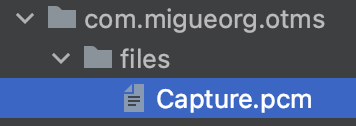
\includegraphics{fotos/archivo_generado.png}
    \caption{Archivo generado.}
\end{figure}

Por lo que a la hora de reproducirlo habrá que especificar manualmente la
velocidad de muestreo o \emph{samplerate}, profundidad de bits y los canales de
audio que tiene la pista \cite{audio-samplerate}, los cuales normalmente vienen
incrustados en las cabeceras de los formatos de audio procesado.

\begin{figure}[H]
    \centering
    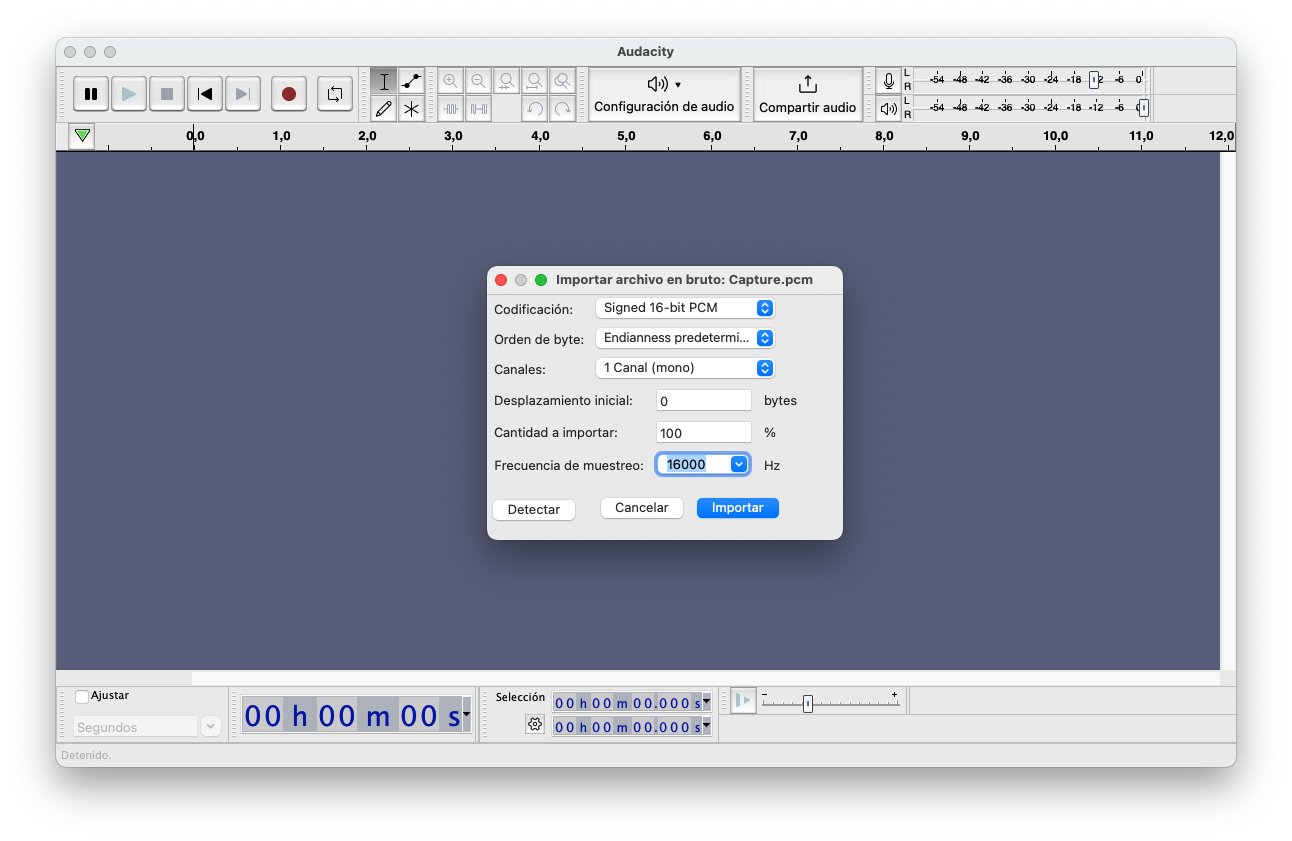
\includegraphics[width=0.9\textwidth]{fotos/importando_datos_en_bruto_audacity.png}
    \caption{Especificando la composición del audio.}
\end{figure}

Sin embargo, puesto que dichos ficheros con extensión pcm no serán empleados para
el uso final, sino que serán utilizados únicamente durante el desarrollo
para verificar que se está capturando el audio y que satisface el PMV (producto
mínimamente viable); esto no es un inconveniente que haya que tener en
consideración más allá que en el de especificar los datos de codificación a la
hora de abrir el archivo generado. 

Por tanto, una vez generado el fichero con
extensión \emph{pcm} con la captura del audio, lo reproduciré para comprobar si
se satisface el PMV. 

\begin{figure}[h!]
    \centering
    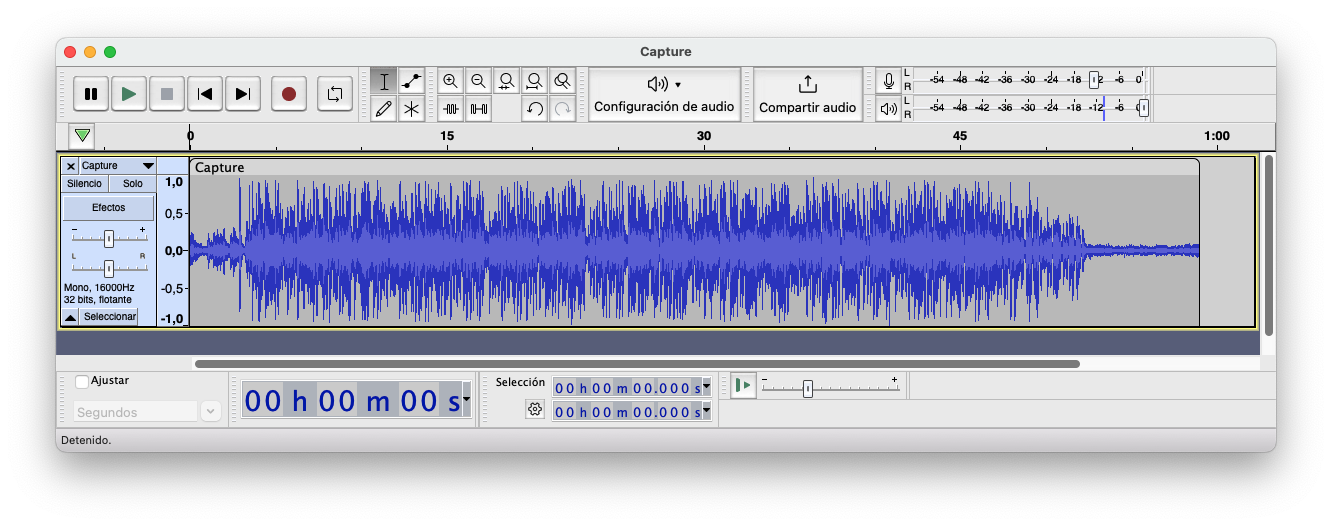
\includegraphics[width=0.9\textwidth]{fotos/muestra_captura_audacity.png}
    \caption{Muestra del audio correctamente capturado.}
\end{figure}

Finalmente, si usamos un software compatible con audio en \emph{RAW} como es
\emph{Audacity} \cite{software-audacity}, vemos que el audio ha sido capturado
correctamente y que es reproducible, por lo que, podemos dar como listo el
milestone 2 al tener satisfecho el PMV asignado al mismo. 


\section{Desplegando el receptor de audio: Milestone 3}

Como ya mencioné al inicio de la implementación, el receptor de audio sería un
dispositivo que corra \emph{Linux}, ya que esto abriría muchas posibilidades en
cuanto a lenguajes y librerías disponibles; por lo que realmente la elección de un
hardware u otro es indiferente mientras ejecute \emph{Linux} y tenga algún
módulo NFC conectado, por ello es que no se ha necesitado un proceso de
selección para este apartado.

En mi caso emplearé una \emph{Raspberry Pi 1b} debido al bajo coste de la misma, su
extensa comunidad y sus puertos de entrada y salida de propósito general
\emph{(GPIO)} \cite{raspberry-gpio} los cuales de cara al desarrollo abren
las puertas a muchos protocolos de manera fácil y rápida. 

\begin{figure}[h!]
    \centering
    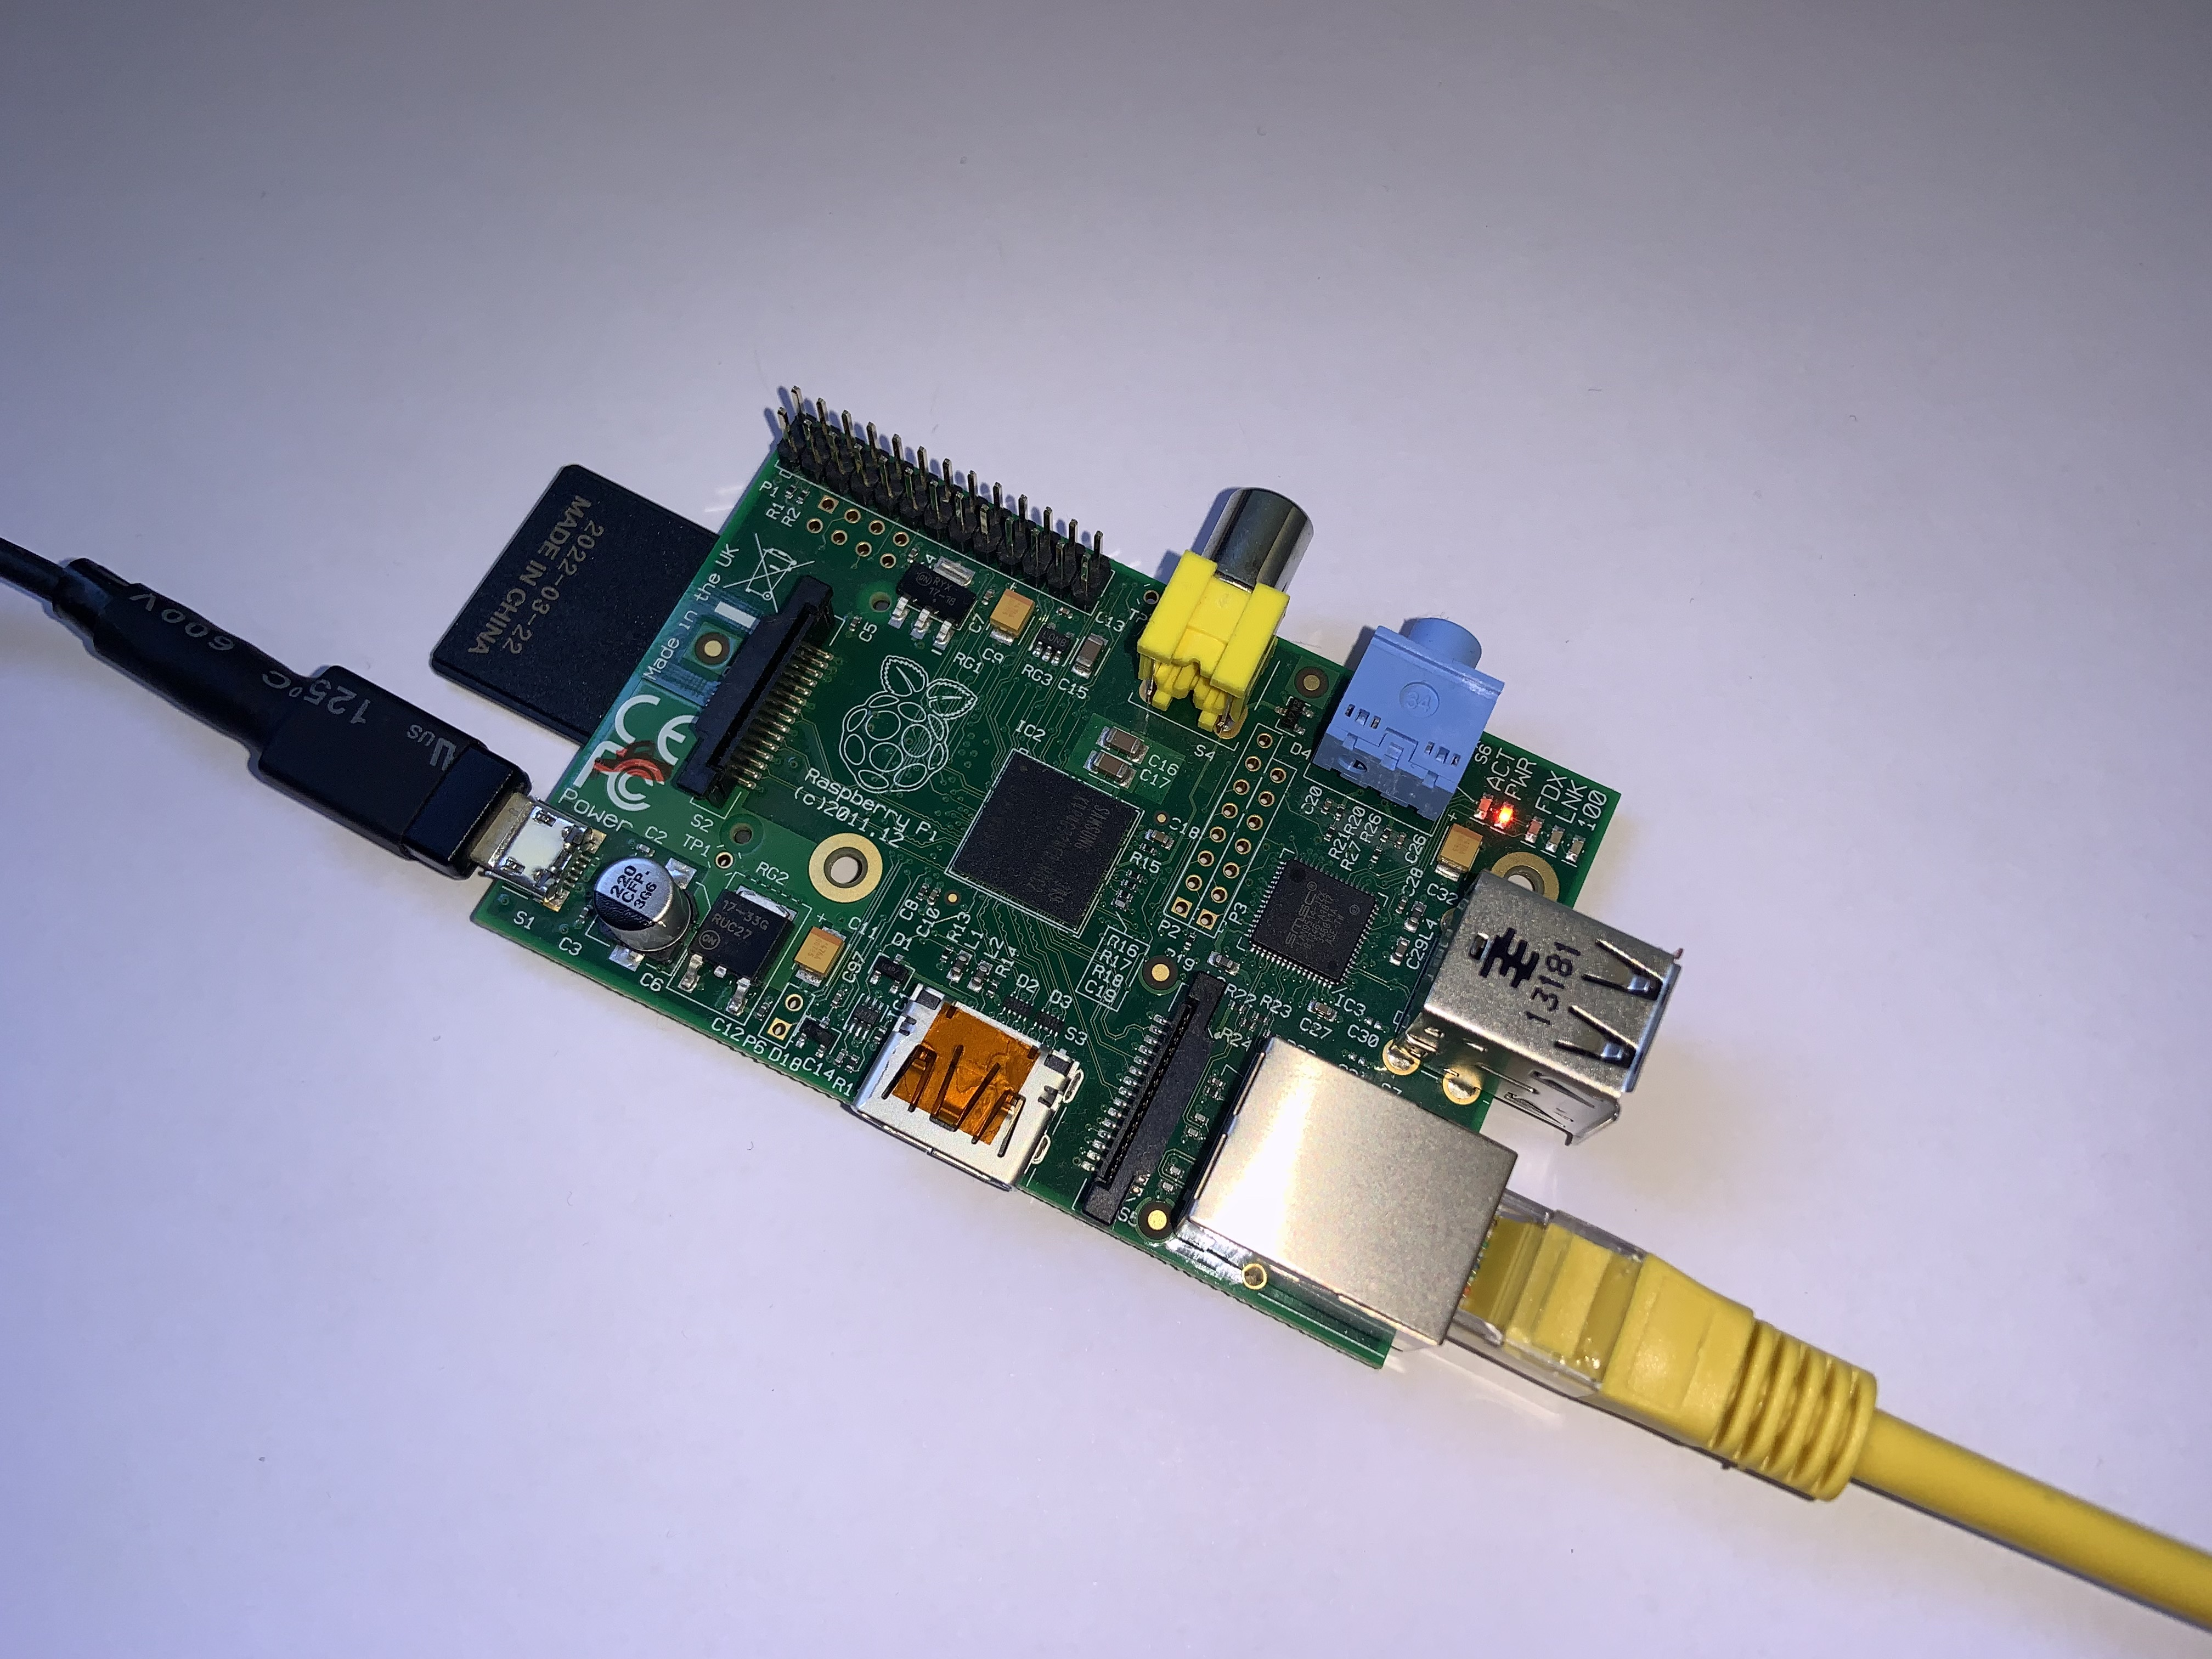
\includegraphics[width=0.8\textwidth]{fotos/raspberry_pi_1b.jpeg}
    \caption{Raspberry Pi 1b.}
\end{figure}

En cuanto al módulo NFC opté por un chip PN532 \cite{raspberry-pn532}, el cual
tiene un bajo coste y su vez admite varios protocolos de conexión diferentes con
la Raspberry Pi.

\begin{figure}[H]
    \centering
    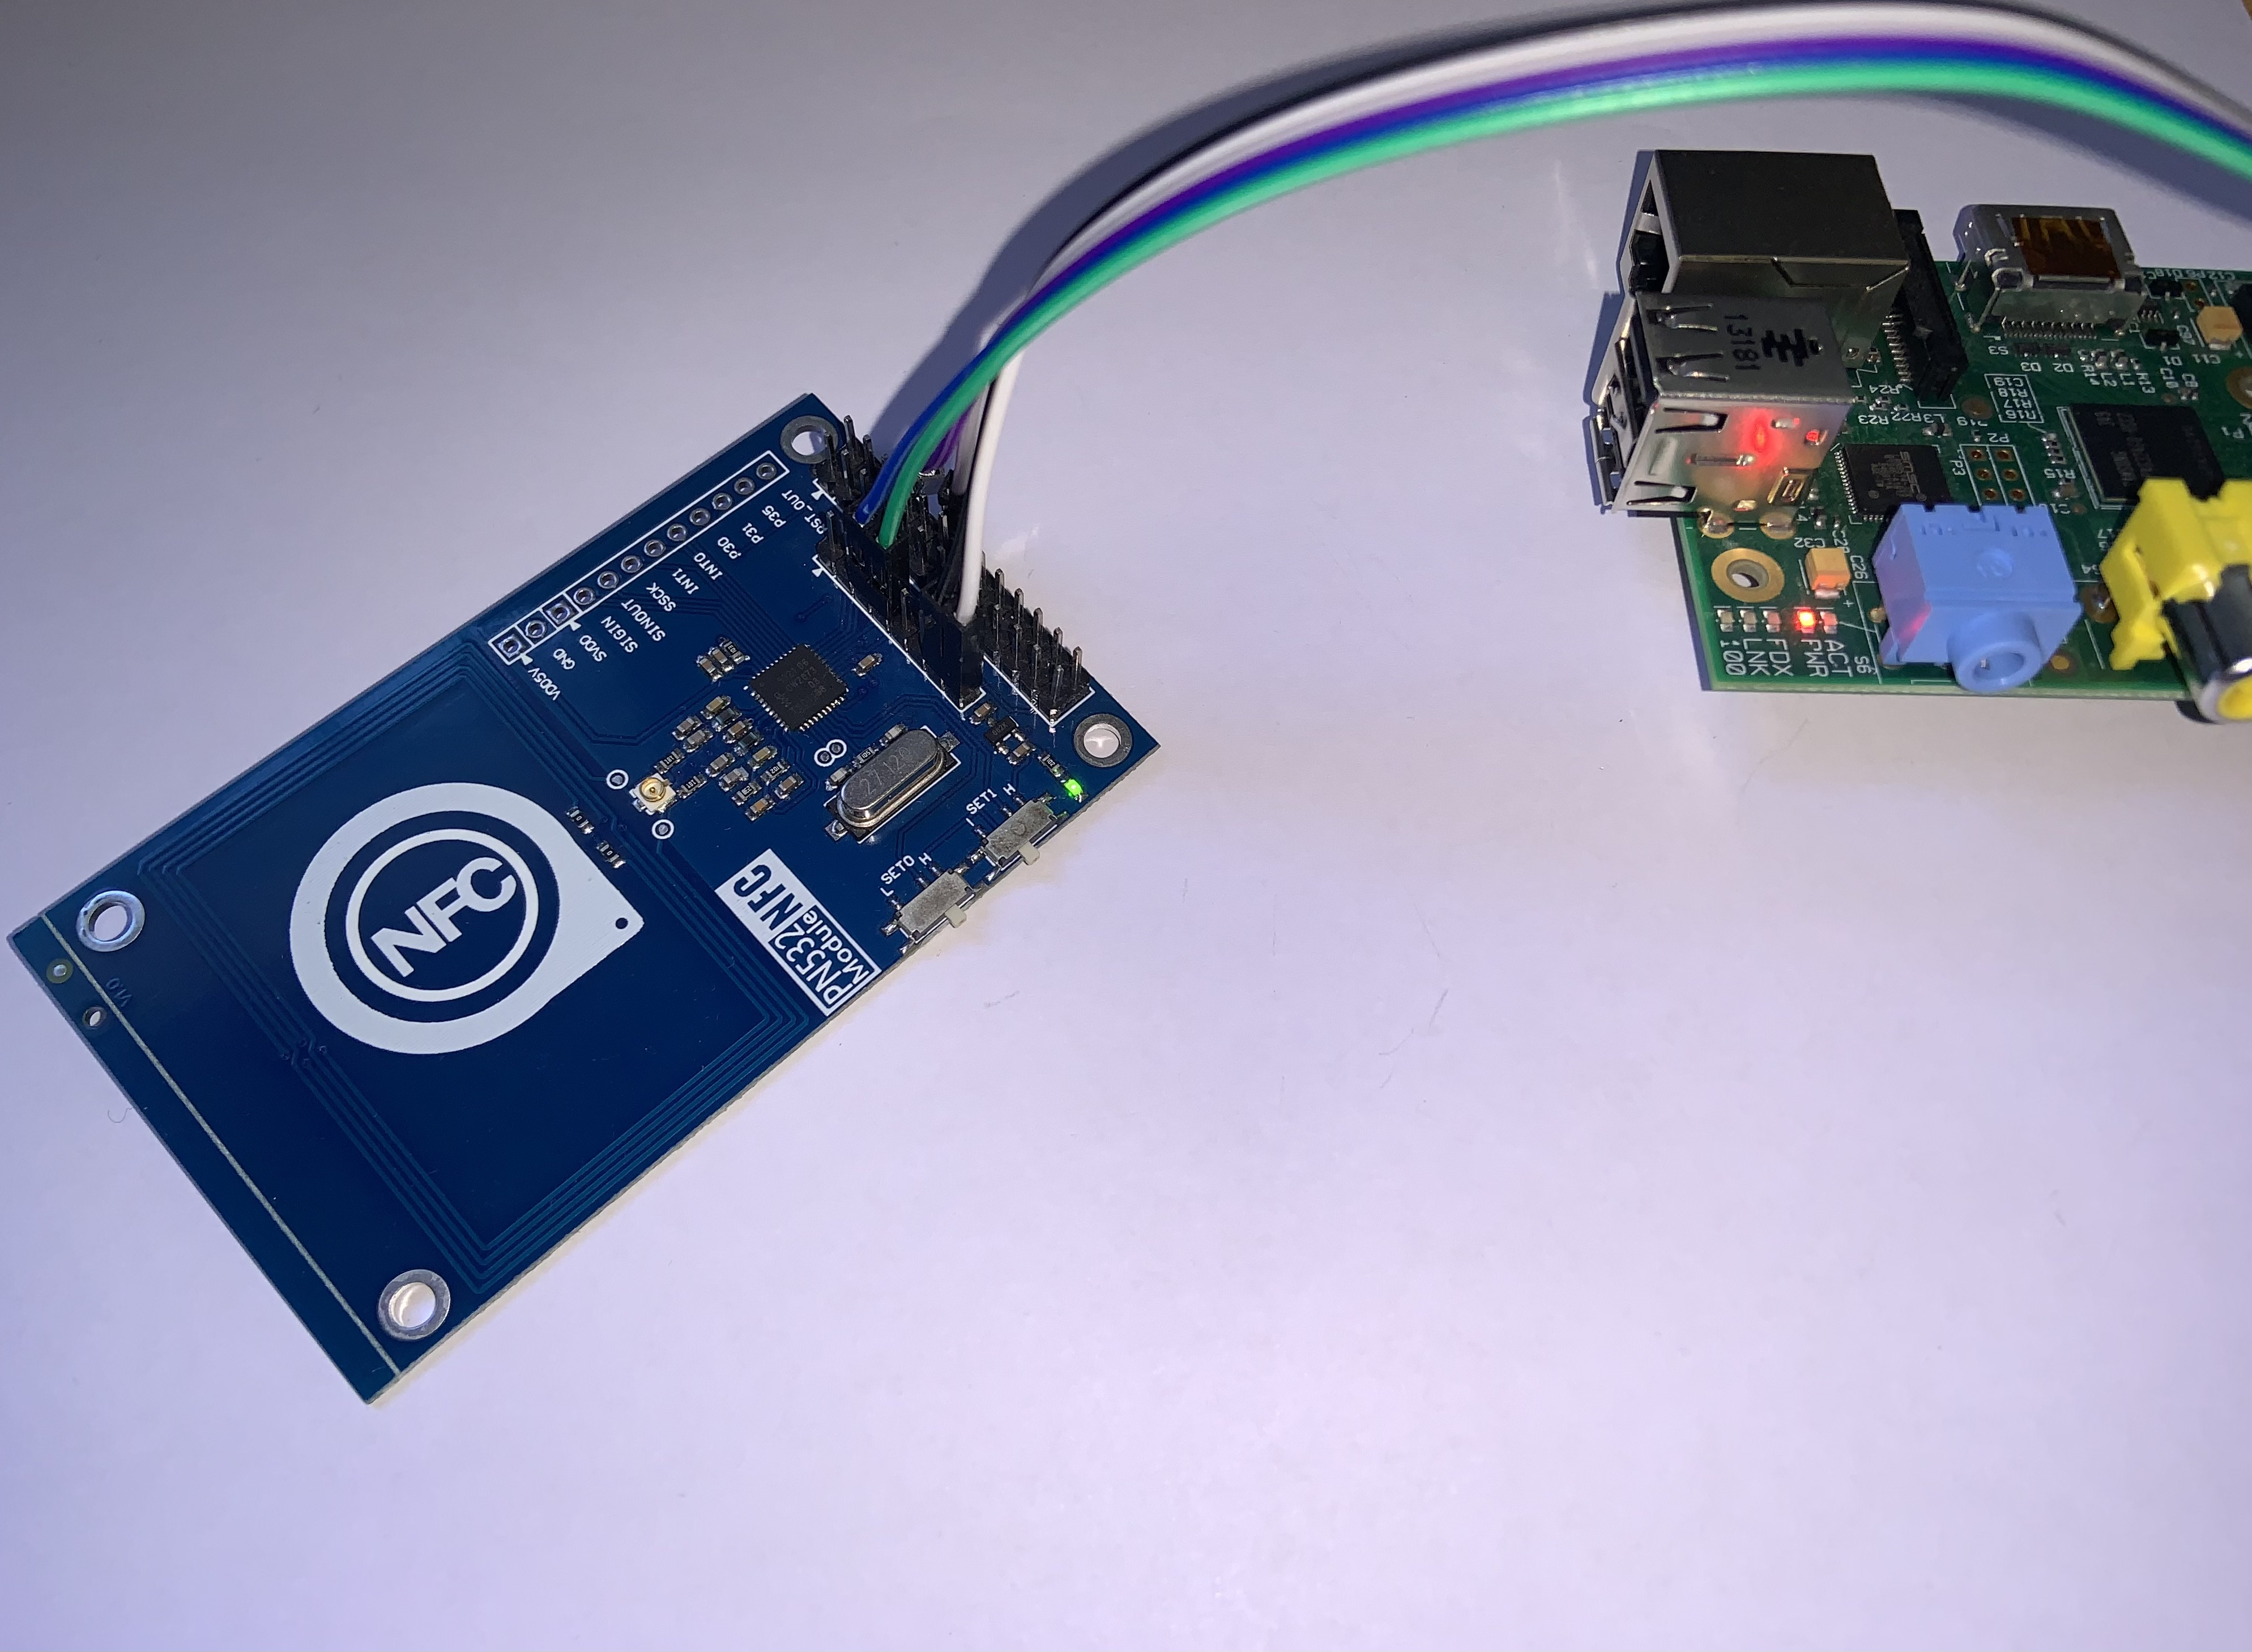
\includegraphics[width=0.7\textwidth]{fotos/pn532_bad.jpeg}
    \caption{PN532 conectado a la Raspberry Pi 1b.}
\end{figure}

Hacer funcionar un chip PN532 en una Raspberry Pi o Arduino es una tarea
sencilla y trivial, sin embargo, durante el desarrollo, tras instalar todo lo
necesario, configurar los drivers y conectar ambos dispositivos; la Raspberry Pi
seguía sin detectar el módulo, independientemente del protocolo de conexión
usado. Por lo que sustituí la Raspberry Pi 1b que estaba utilizando por otra
Raspberry Pi 2. 
Pero el resultado seguía siendo el mismo incluso después de reinstalar el
sistema y reinstalar los drivers desde cero en la nueva Raspberry Pi. Por lo que
sustituí el módulo PN532 por otro de un fabricante diferente, en este caso uno de
\href{https://www.waveshare.com/wiki/PN532_NFC_HAT}{Waveshare}

\begin{figure}[hb]
    \centering
    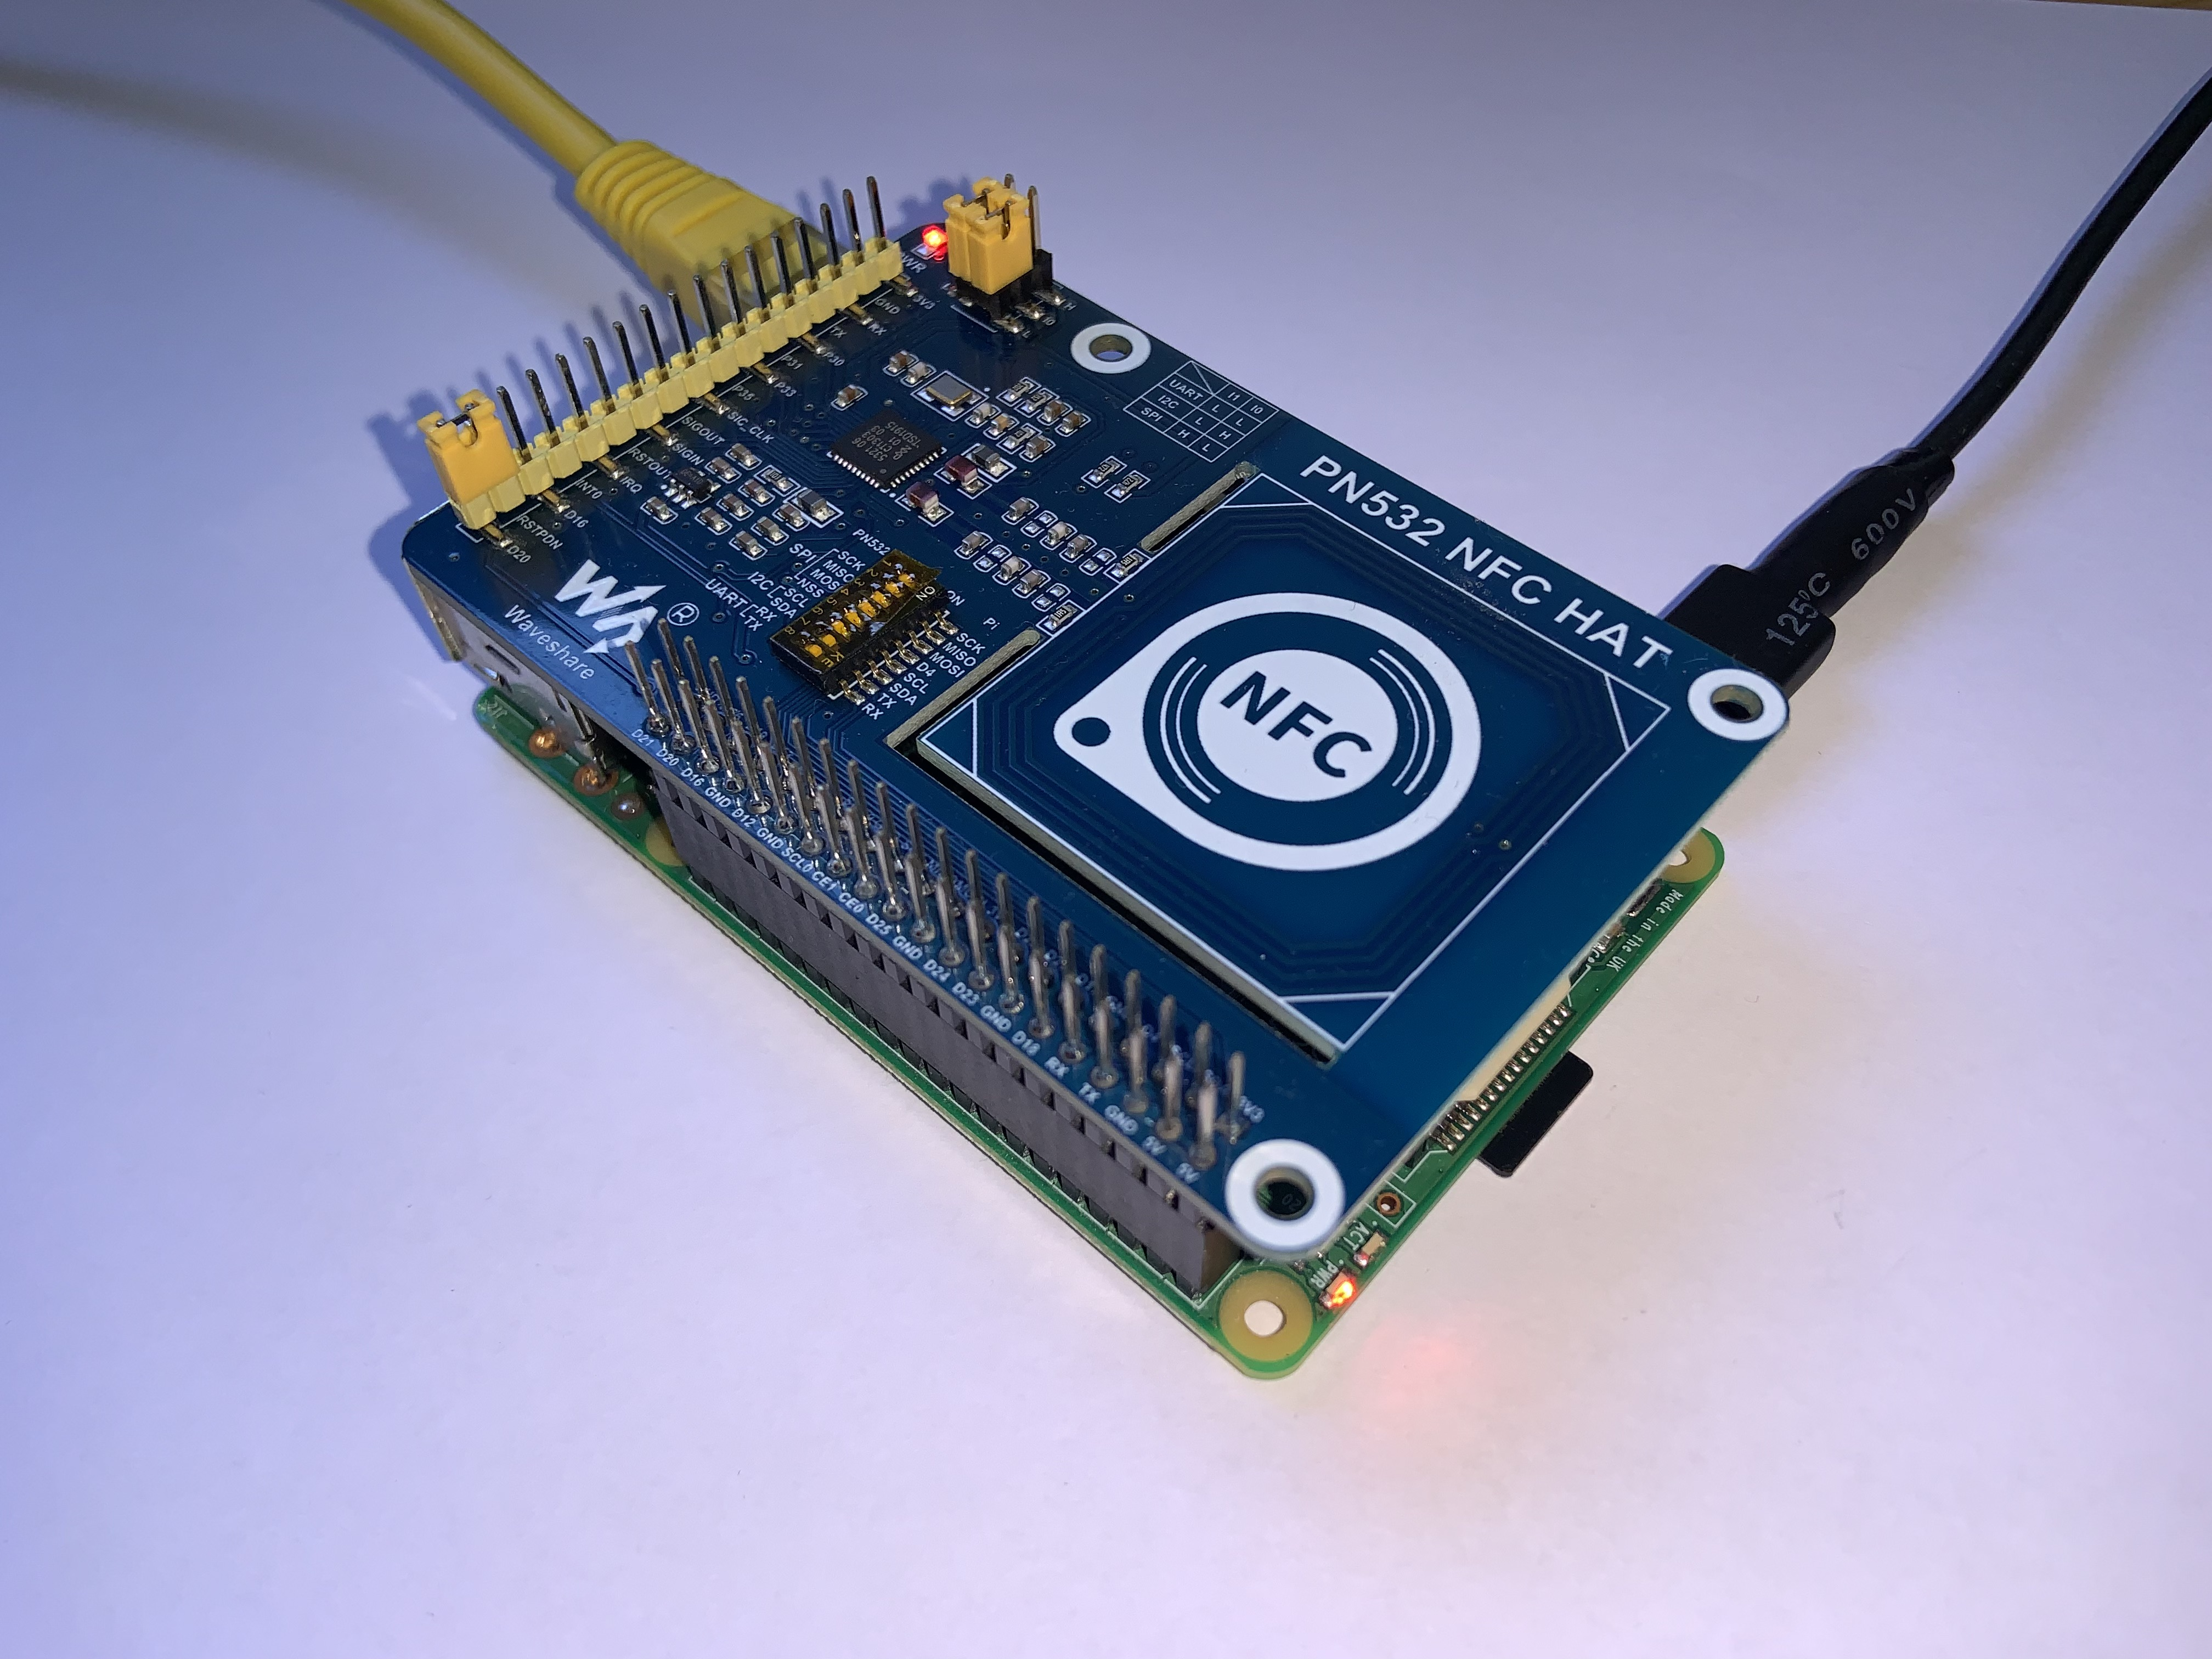
\includegraphics[width=0.7\textwidth]{fotos/pn532_good.jpeg}
    \caption{Nuevo PN532 de Waveshare con formato \emph{HAT} conectado a la Raspberry Pi 2.}
\end{figure}

El cual finalmente sí que funcionó por lo que saqué como conclusión que el primer
módulo PN532 llegó roto. Lo cual provocó una semana de trabajo perdido entre
pruebas, intentos y tiempos de espera.

\begin{figure}[ht]
    \centering
    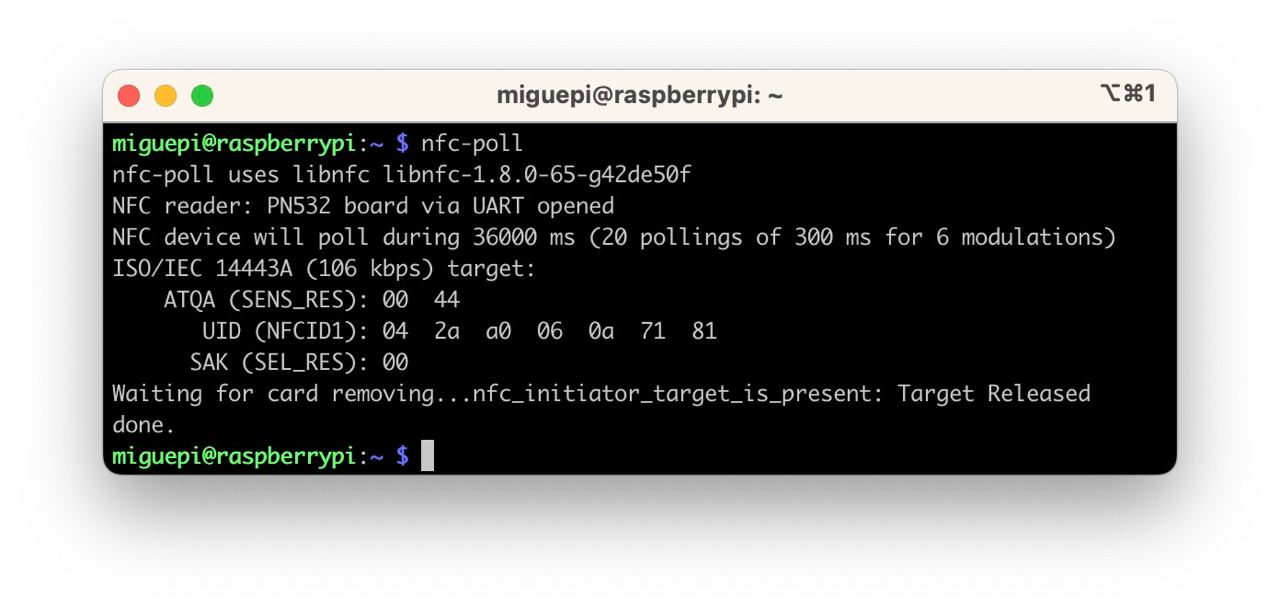
\includegraphics[width=\textwidth]{fotos/nfc_poll.jpeg}
    \caption{nfc-poll detectando el PN532 via UART en la Raspberry Pi 2.}
\end{figure}

Para conectar un módulo PN532 a una Raspberry Pi, como mencioné antes, existen
varios protocolos disponibles, los cuales son \emph{UART}, \emph{I2C} y
\emph{SPI}. Sin embargo, tras hacer un estudio de los protocolos compatibles con
la librería \emph{NFC} seleccionada tras un proceso de selección al inicio,
comprobé que el único protocolo compatible con la misma era el de \emph{UART}
(conexión serie), por lo que tampoco fue necesario realizar un proceso de
selección sobre los protocolos disponibles.\\

Una vez operativa la Raspberry Pi y el módulo \emph{NFC}, instalé los lenguajes
elegidos en los procesos de selección que se llevaron a cabo, además de la
librería \emph{NFC (NfcPy)} seleccionada, los cuales no presentaron ningún
problema. Por lo que tras esto, el despliegue y configuración del dispositivo
receptor ya se encontraba listo.


\section{Comunicación entre dispositivo móvil y receptor: Milestone 4}

Esta ha sido con diferencia la parte del desarrollo donde hemos tenido que
aplicar más a fondo metodologías de programación para poder superar los retos

Para empezar con el desarrollo, este milestone se puede dividir a su vez en 4
objetivos, de los cuales 2 y 2 irán de la mano. Envío de audio en la parte del
móvil, recepción de audio en la parte del receptor para el módulo del streaming
de audio; así como lectura de NFC por la parte del dispositivo móvil y escritura
NFC por la parte del receptor para el módulo de NFC.

\subsection{Transmisión de audio entre móvil y receptor}

En una primera instancia se propuso enviar el audio capturado mediante algún
protocolo pensado y dedicado al streaming, como pueden ser WebRTC
\cite{protocolo-webrtc}, RTSP \cite{protocolo-rtsp}, HLS \cite{protocolo-hls},
etc. los cuales a día de hoy son ampliamente usados y conocidos. Sin embargo, se
presentó el primer problema; estos no son compatibles con audio en
\href{https://en.wikipedia.org/wiki/Raw_audio_format}{RAW} (sin procesar). Cada
uno de estos protocolos tienen una lista de codecs soportados para audio y
video \cite{protocolo-codecs}, cuya lista es más bien escasa, soportando nada más que un par de codecs
cada uno, pero por supuesto, nada de audio sin procesar en ninguno de estos
protocolos.\\

Para poder utilizar estos protocolos ideales de streaming, habría que añadir una
codificación en tiempo real al audio, lo cual consumiría una cantidad elevada de
recursos adicionales y batería al dispositivo, además de añadir una latencia
extra en el audio. Por supuesto, también requeriría el uso de bibliotecas
externas, ya que Android de forma nativa no tiene soporte para codificar ciertos
formatos como podría ser MP3 (lo tiene para decodificar, no obstante, no para
codificar) \cite{android-mp3}. Lo cual también llevaría un tiempo de desarrollo extra, pues habría
que realizar el proceso de estudio y selección correspondiente sobre las
bibliotecas existentes.\\

Debido a esto, y con el fin de evitar tener que codificar en tiempo real todo el
audio interno, se ha optado por emplear un socket \cite{protocolo-socket} y tratar el audio como si
fuese un archivo a enviar en lugar de emplear alguno de los protocolos ya
mencionados.\\

A la hora de crear un socket \cite{protocolo-socket} existen dos posibilidades,
emplear el protocolo TCP \cite{protocolo-tcp} o UDP \cite{protocolo-udp}:

\begin{itemize}
    \item El protocolo TCP es orientado a conexión, por lo que incorpora un
    control de paquetes y de pérdidas, que asegura el correcto envío, recepción
    de manera ordenada y negociación de los mismos. Esto hace que cuando
    hablemos del envío de archivos de gran tamaño, la red se vea más saturada,
    pues dicho control de sesión agrega un tamaño a las cabeceras de los
    paquetes y un volumen considerable al aumentar la cantidad de los mismos que
    se precisarán para la transferencia.
    \item El protocolo UDP, por otro lado, no es orientado a conexión, por lo
    que no asegura la recepción de los paquetes, ni incorpora control de
    pérdidas, sin embargo, esto hace que tanto las cabeceras como el volumen de
    paquetes sean mucho menores, pues no necesita llevar a cabo ningún tipo de
    control ni negociación continua, provocando que las velocidades de
    transferencia sean mayores y que, por tanto, el envío y recepción tenga
    menos latencia, aunque puedan presentarse ciertas pérdidas.
\end{itemize}

Es por esto que, dado las necesidades del proyecto de una comunicación en tiempo
real para la reproducción de audio en streaming, se ha optado por implementar un
socket UDP en lugar de TCP.\\

Puesto que UDP no incorpora un control de pérdidas, ni asegura la correcta
recepción de los paquetes; trabajar con ficheros regulares sería un error debido
a la facilidad de corrupción de los mismos en el momento de la pérdida de algún
paquete. Por lo que el fichero con extensión PCM con la captura de audio en RAW
que se creó en el milestone 2 no es válido para este enfoque, así pues, habrá
que enviar el flujo de audio del objeto AudioRecord a través del socket UDP en
lugar de guardarlo en un fichero pcm.\\

Este nuevo enfoque de enviar el objeto de flujo de bytes de audio en lugar de un
fichero regular, provoca que en el lado del receptor, en lugar de recrear y
reproducir el archivo reproducible por cualquier reproductor de audio, haya que
implementar un método que reproduzca sonido a partir de un objeto de flujo bytes
de audio. Para ello existe una clase llamada SourceDataLine en Java
\cite{java-SourceDataLine}, con la cual ya había trabajado en otras asignaturas,
que permite la reproducción de audio a partir de un array de bytes especificando
previamente el formato en el que ese audio ha sido obtenido (frecuencia de
muestreo, canales, etc.) por lo que debido a esto, y tal y como se comentó en
\hyperref[seleccion-streaming-receptor]{el proceso de selección} se decidió
emplear Java en el lado del receptor.\\

Una vez programada la recepción de datagramas socket y la recreación del objeto
de audio, pude comprobar que el streaming era funcional y mantenida en tiempo
real, sin embargo, había muchísimos micro cortes, que llegaban a imposibilitar
la escucha de audio.\\

Para solventar esto se fue variando la frecuencia de muestreo del audio (para
aligerar las muestras de sonido sacrificando calidad) y el tamaño de los
datagramas UDP (para reducir el número de paquetes, aumentando el tamaño de los
mismos y evitar saturar la red).\\

Gracias a esto finalmente se ha conseguido un resultado más aceptable, teniendo
en cuenta las limitaciones, y es que UDP no permite enviar datagramas mayores a
64 kB, por lo que al estar transmitiendo audio sin procesar, se crea un muy alto
volumen de paquetes, lo cual hará muy propensa la pérdida de los mismos. Todo
esto sumado al no tener implementado ningún método para el control de pérdidas,
ni para el dimensionado dinámico de paquetes (como otros protocolos destinados a
streaming si hacen), provocará que ocurran ciertos cortes, y que la calidad de
audio no pueda ser excesivamente alta, pues aumentaría mucho más el tamaño.\\

Sin embargo, a pesar de los micro cortes puntuales y la disminución de la
calidad, la transmisión es estable, a tiempo real y sin retardo en el audio
(ante unas mínimas condiciones de red aceptables), por lo que los objetivo de
envío y recepción de audio cumplen los requisitos para un PMV.

\subsection{Comunicación NFC entre móvil y receptor}

Dado que la transmisión de audio va a través de la red, el uso de NFC se reduce
a dos funciones: 

\begin{itemize}
    \item Iniciar la actividad de captura de audio y transmisión del mismo.
    \item Identificar a que dispositivo se debe de transmitir el audio.
\end{itemize}

Así pues, para una tarea tan simple, la lista de tecnologías candidatas es
amplia. Por ello, se llevó a cabo un análisis de las posibles alternativas para
realizar las dos tareas que se mencionaron antes, la cual acabó resultando
en el NFC como mejor vía posible.

\subsubsection{Eligiendo la tecnología a usar}

En primera instancia, si nos fijamos en el \hyperref[estado_del_arte]{estado del arte}, la opción que más se
acerca a la solución del problema es \hyperref[solucion_apple]{la que implementa \emph{Apple}}, por lo que
analizando su forma de llevar a cabo las dos tareas iniciales, descubrí que lo
hacen a través de su chip llamado \emph{Apple U1}; el cual no es más que un chip
de \emph{UWB} \cite{uwb-explicado} de fabricación propia, cuyo fin es el de
posicionar espacialmente sus dispositivos, tal y como vemos que hacen con los
\emph{Apple AirTags}. De esta manera, gracias a este chip, saben cuando un
dispositivo está al lado de otro con mucha precisión, ya que no solo pueden
conocer la distancia entre ambos, sino también la orientación de los mismos. Así
pues, gracias a dicho chip, saben cuando un \emph{iPhone} está tocando a un
\emph{HomePod}, para a continuación iniciar el \emph{streaming} de audio. Sin
embargo, el empleo de esta tecnología para un proyecto destinado a
\emph{Android} no es algo viable, pues a pesar de que el \emph{UWB} no es una
tecnología propietaria o exclusiva de \emph{Apple}, esta no está presente
normalmente en \emph{Android}, de hecho, únicamente está presente en un total de 8
dispositivos \cite{uwb-android}. \\

Valorando otras tecnologías existentes en (al menos) la gran mayoría de
dispositivos \emph{Android} encontramos el wifi y el bluetooth. El problema es
que estas tecnologías tienen un gran alcance, y es por esto que no son ideales
para emplearlas en técnicas de posicionamiento a escasos centímetros, lo cual es
lo que se está buscando. La elección de las mencionadas tecnologías provocaría que se
activase en ocasiones en las que realmente no se desea. Además, son redes que
por lo general suelen estar ocupadas para otros fines, por lo que el empleo de las
mismas para este proyecto podría interferir con el uso real del dispositivo (por
ejemplo tener que desconectarse del wifi para usarse, etc.).\\

Sin embargo, dentro de la familia del \emph{Bluetooth}, existe una variante
denominada \href{https://en.wikipedia.org/wiki/Bluetooth_Low_Energy}{BLE
\emph{(Bluetooth Low Energy)}}, la cual es una derivación del propio
\emph{Bluetooth} tradicional, pero enfocado en un bajo consumo de energía,
sacrificando el alcance y velocidad. Esta tecnología permite varias clases de
funcionamiento dentro de \emph{BLE}, donde la clase 4 del mismo (el más bajo)
establece un alcance de medio metro. Sin embargo, medio metro sigue
pareciendo demasiada distancia como para que pueda activarse involuntariamente.
Además, también hay que tener en cuenta con que el descubrimiento \emph{Bluetooth} suele
precisar unos segundos, sin contar con los que además sean necesarios en la
propia comunicación. Haciendo que esta tecnología quede descartada.\\

Finalmente, encontramos el ya conocido e involucrado a diario para pagos,
\href{https://es.wikipedia.org/wiki/Comunicaci%C3%B3n_de_campo_cercano}{NFC}, 
el cual si bien no está tan expandido en móviles como el \emph{Bluetooth}, a día
de hoy ya es raro encontrar dispositivos \emph{Android} que carezcan de esta
tecnología. El \emph{NFC} tiene un alcance que va desde escasos milímetros hasta
no más de 20cm y no requiere tiempo de descubrimiento pues en cuanto existe el
contacto se inicia la comunicación, lo cual lo convierte en una alternativa
viable para emplearla en este proyecto. 

\subsubsection{Implementando la transferencia}

En los primeros planteamientos del proyecto se propuso que el móvil enviase la
URL del \emph{streaming} al receptor por NFC, sin embargo, el uso de
\emph{sockets} eliminó esa necesidad; por lo que la única información necesaria
era la de conocer por parte del dispositivo móvil, la dirección IP del
\emph{socket} al que enviar los paquetes. Así pues, lo necesario a implementar
era el anunciado de la IP del receptor, y la lectura de la misma por parte del
dispositivo móvil.\\

Como primer acercamiento, utilicé la ya presentada biblioteca NFC para Python,
nfcpy para enviar la dirección IP del receptor. Para ello, empleé los archivos y
comandos de ejemplo que proporcionan para casos simples, como era el de enviar
texto por NFC a través de
\href{https://nfcpy.readthedocs.io/en/latest/examples/beam.html}{beam}. Sin
embargo, este método \emph{send} presentaba un error en la negociación inicial
con el teléfono al acercarlo, por lo que no llegaban a realizar ninguna
transferencia. Y dado que \emph{Google} discontinuó la \emph{API} de
transferencia de archivos mediante NFC llamada \emph{Android Beam} en Android 10
\cite{android-beam-deprecated}, supuse que podrían tener relación, por lo que
decidí buscar otro camino evitando la transferencia de archivos.\\

Para un siguiente enfoque, propuse que en vez de efectuar una transferencia con
la que enviar la IP al móvil, esta fuese una simple lectura, al igual que cuando
se lee una etiqueta simple de NFC, cuyo funcionamiento y compatibilidad sí que
están disponibles aún en \emph{Android}. El problema es que la biblioteca nfcpy
permite leer y escribir dichas etiquetas, pero no simular una etiqueta al gusto.
Sin embargo, una función que si implementa esta biblioteca y que se acerca a
esta solución es la de emular una tarjeta NFC, para la cual es necesario cargar
un archivo con extensión \emph{ndef}, el cual debe contener el volcado de la
memoria de una etiqueta NFC, es decir, cabeceras y mensaje. De esta forma, sería
posible emular una tarjeta NFC, de la cual el \emph{Android} sí que podría leer
fácilmente.\\

De nuevo, el siguiente problema fue que no hay ningún volcado de la memoria de
una tarjeta NFC público por internet, ni algún archivo \emph{ndef} descargable
que usar como plantilla, por lo que, lo que tuve que hacer fue conseguir unas
etiquetas o tarjetas NFC vírgenes, las cuales usando la biblioteca nfcpy,
gracias al flag ``dump'', pude hacerles un volcado de la memoria, y a partir de
los cuales obtener un archivo \emph{ndef} que poder emular.\\

\begin{figure}[H]
    \centering
    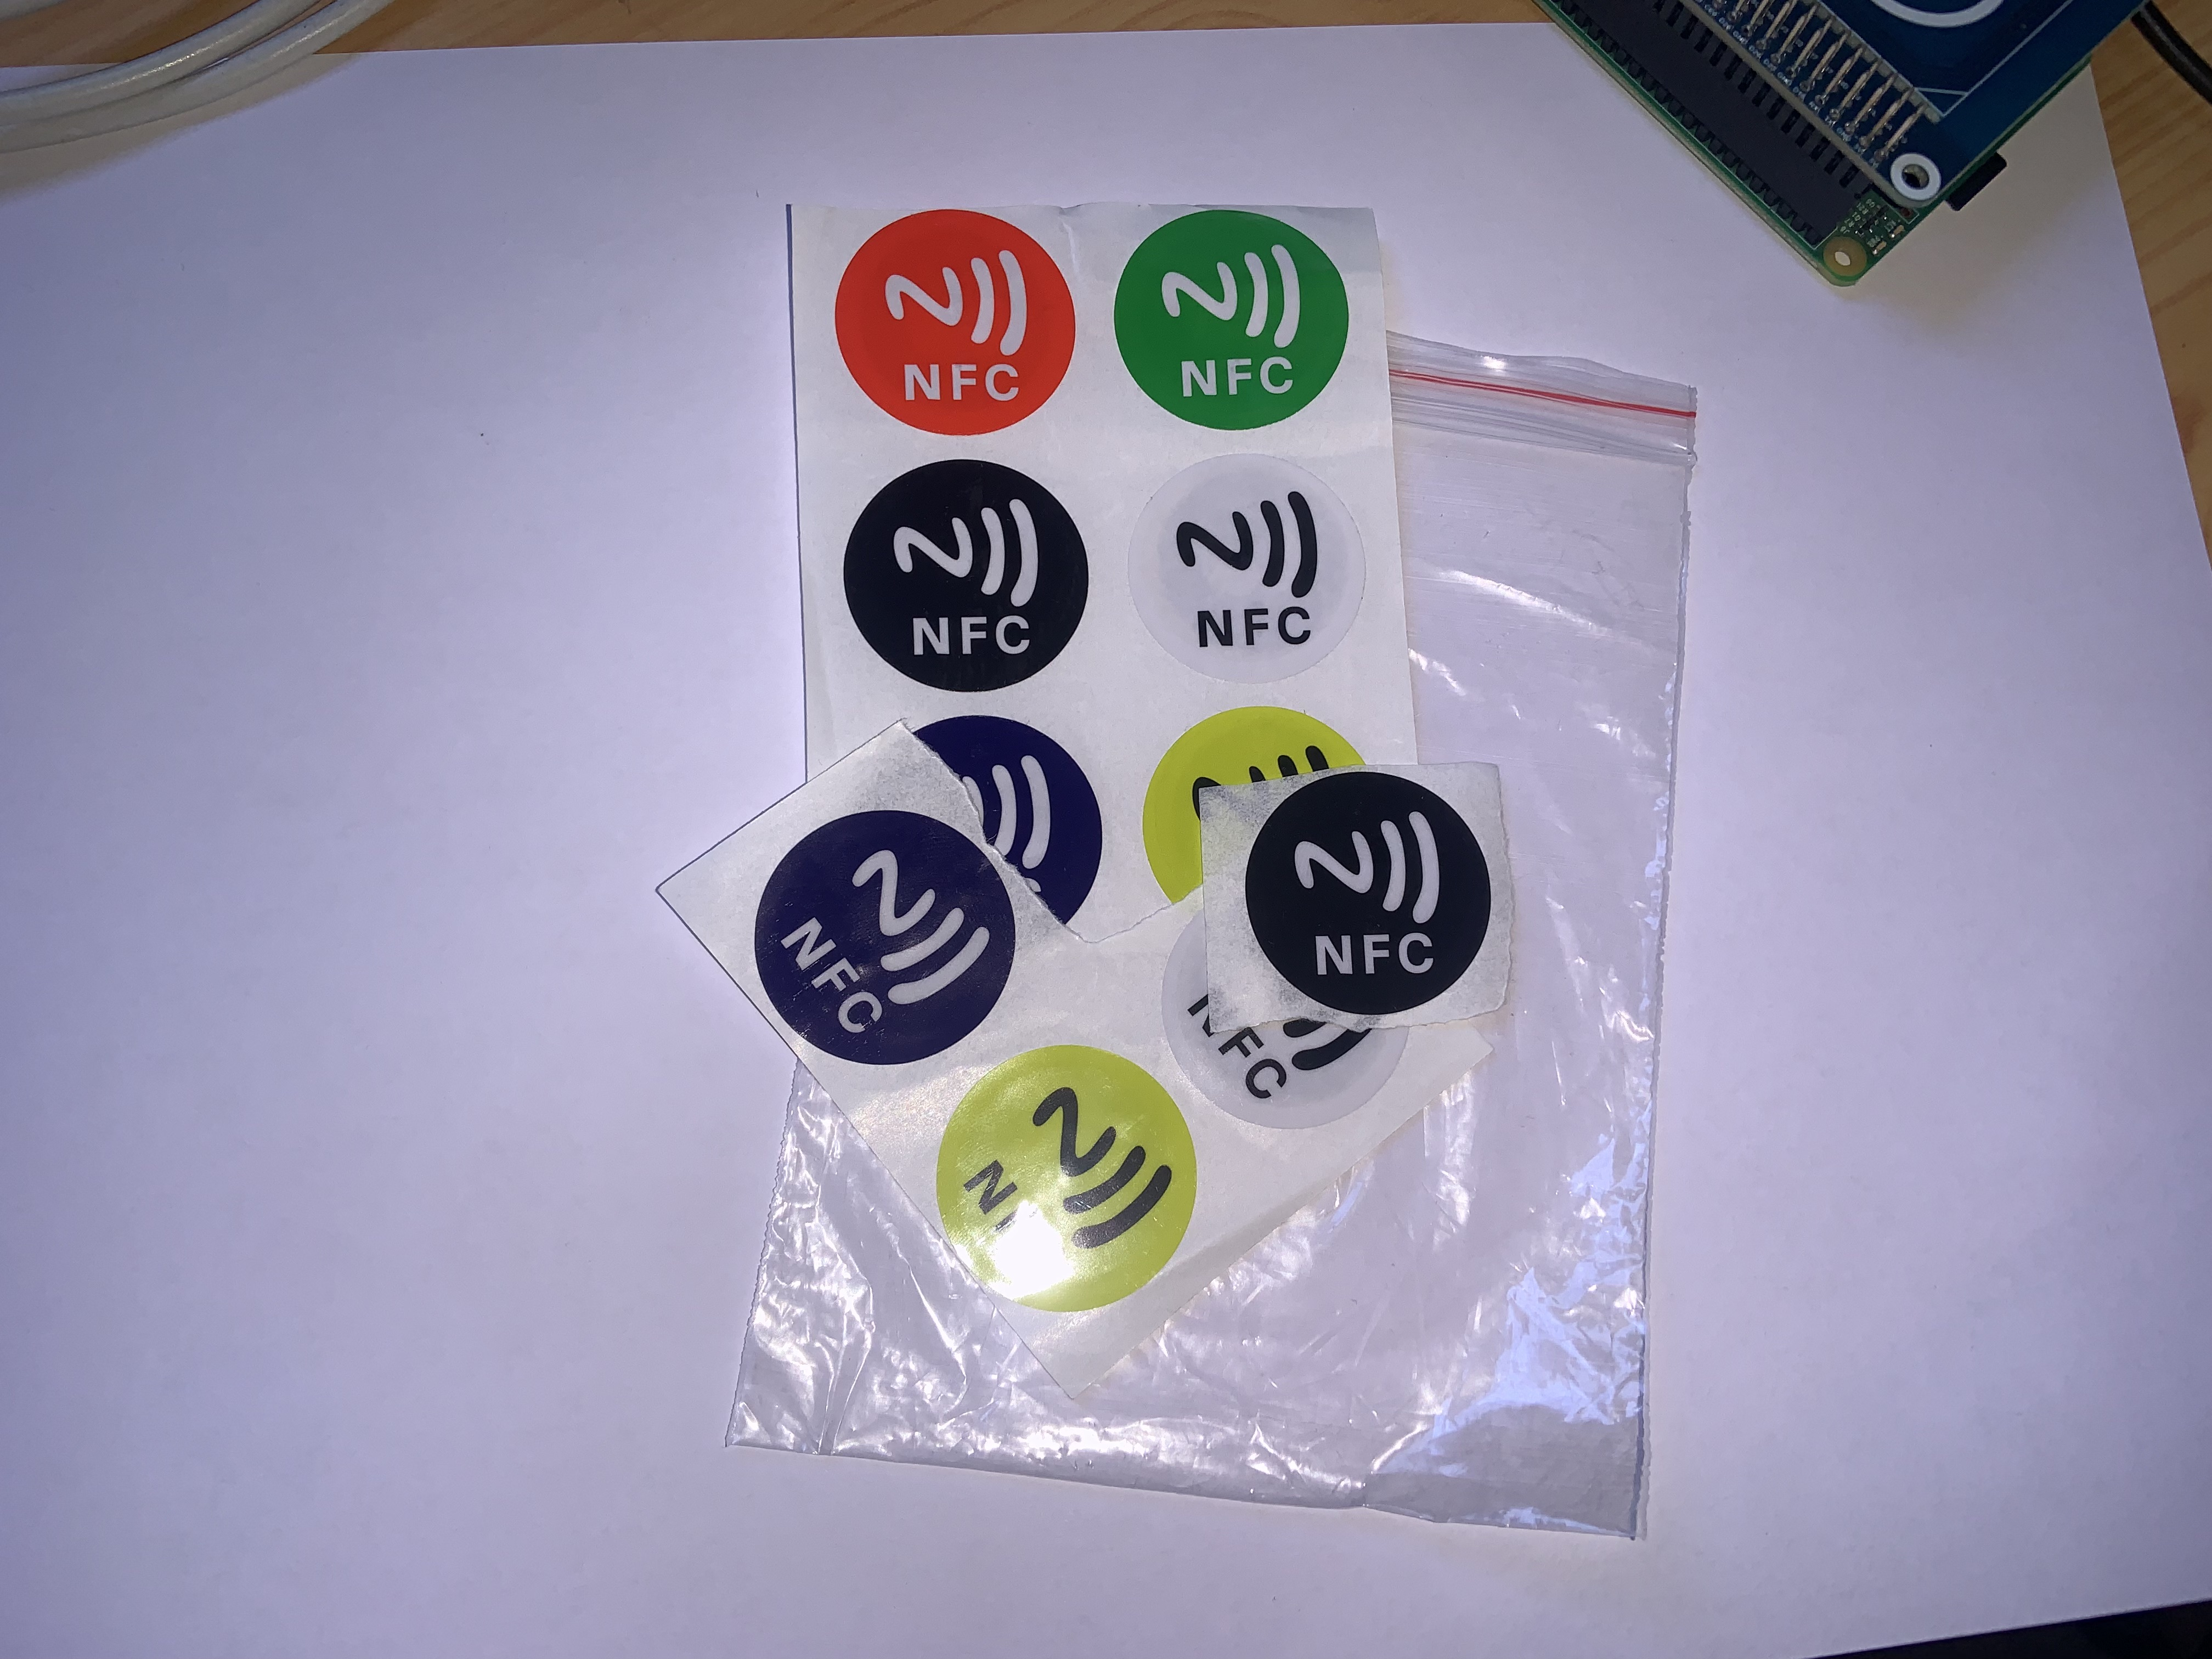
\includegraphics[width=0.65\textwidth]{fotos/etiqueta_nfc.jpeg}
    \caption{Etiquetas NFC vírgenes.}
\end{figure}

Esto funcionó, ya que con ese archivo \emph{ndef} extraído, la Raspberry Pi
emuló la tarjeta \emph{NFC}, pero el problema era que se emulaba con la
información que tuviese en el momento del volcado de la etiqueta, por lo que no
me permitía reescribir la información que tuviese escrita, o seleccionar un
mensaje diferente.

Por lo que el siguiente paso fue el de hacerle ingeniería inversa a la memoria de
las etiquetas para ver como almacenaban la información, y así poder crear un
archivo ndef al gusto. Para esto, fui reescribiendo etiquetas \emph{NFC}, variando
ligeramente el mensaje entre ellas, volcar la memoria de las mismas usando nfcpy
y abriendo los \emph{dump} de las mismas con un visor hexadecimal como
\href{https://hexed.it/}{HexEd.it}.

\begin{figure}[H]
    \centering
    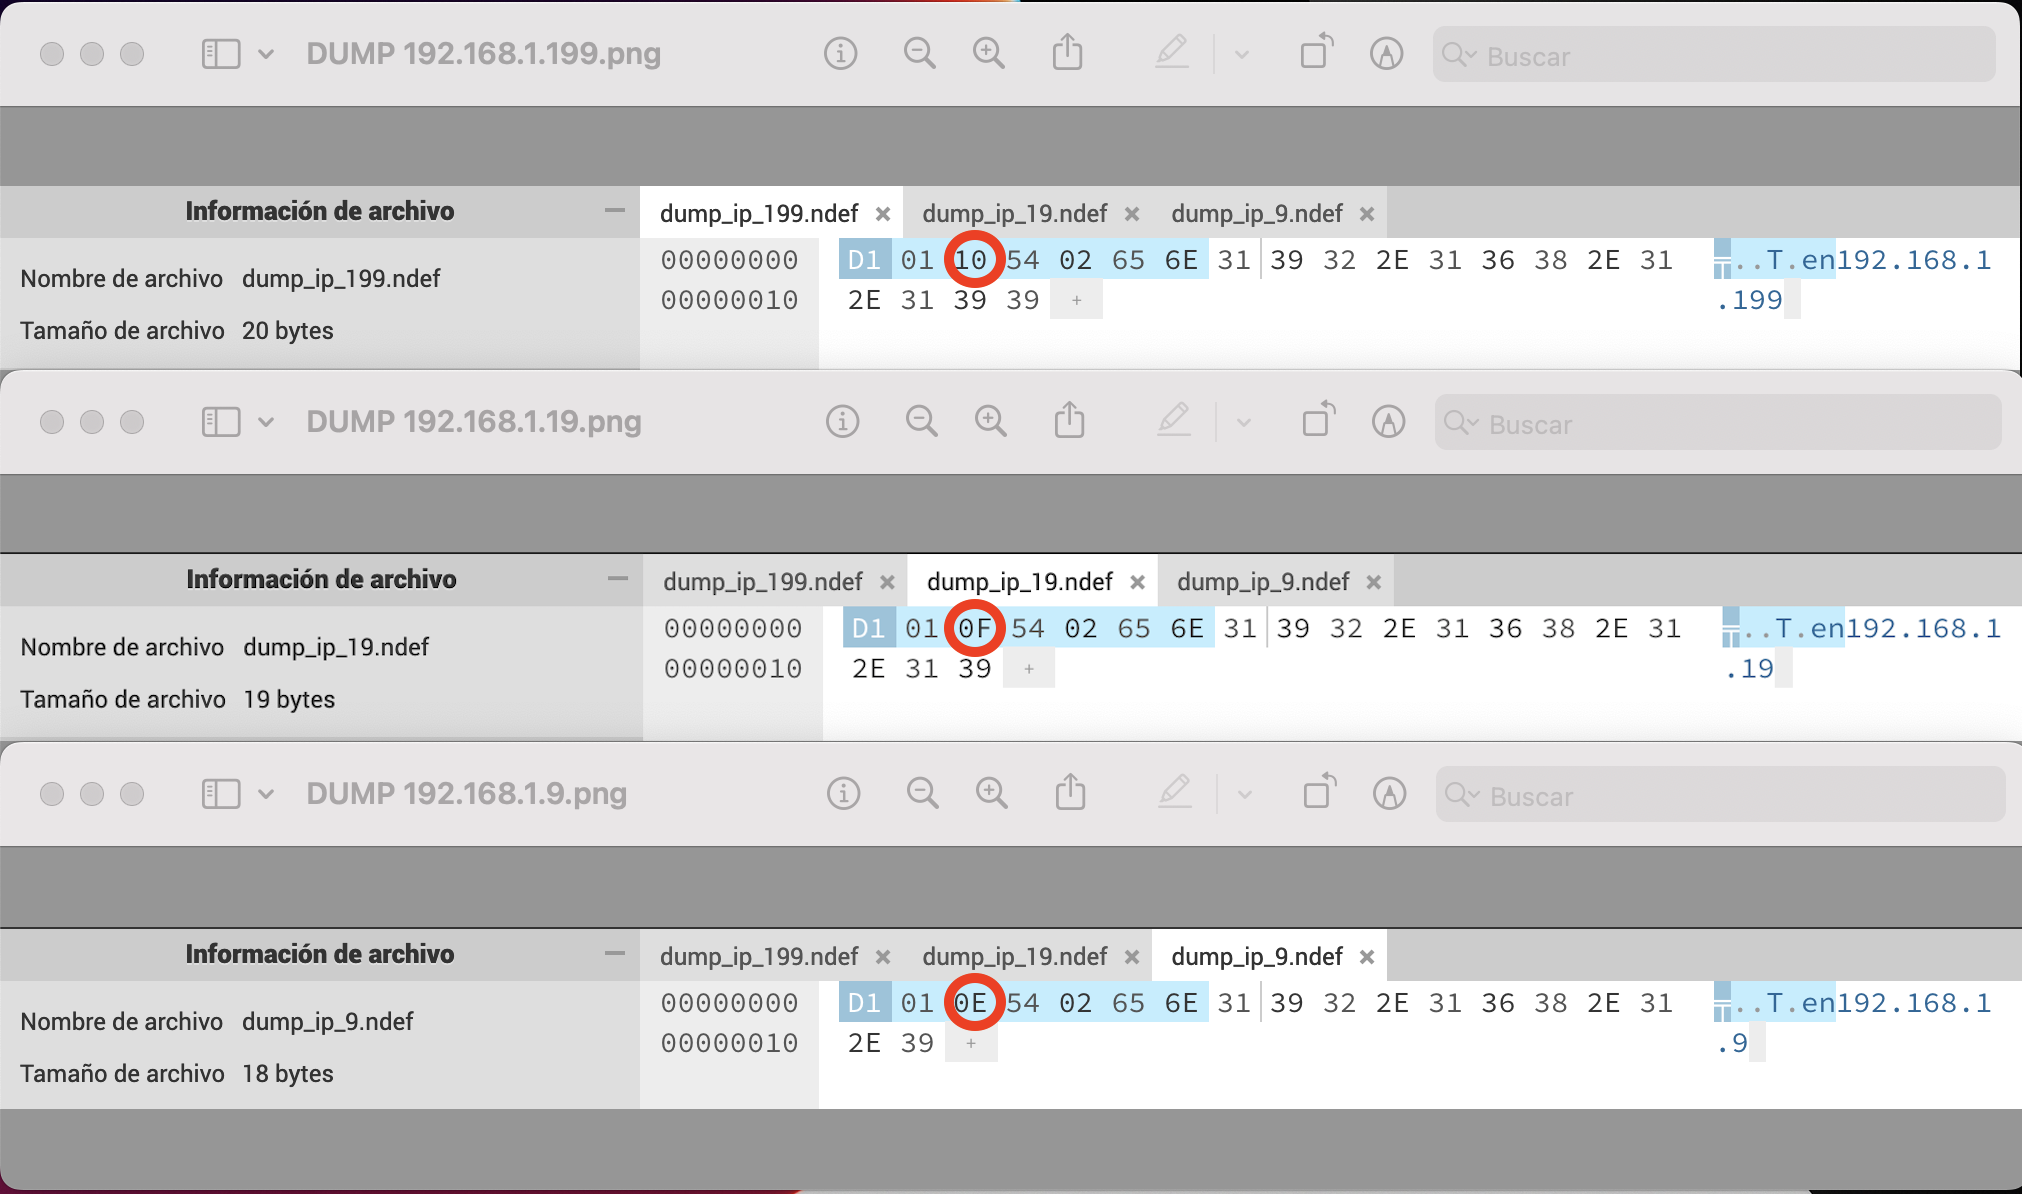
\includegraphics[width=\textwidth]{fotos/muestra_dumps.png}
    \caption{Cambios en la cabecera de varias muestras.}
\end{figure}

Tras analizar varios volcados de memoria y entender la estructura interna de
\emph{NDEF} \cite{ndef-explicado}, pude apreciar que los primeros 7 bytes son
dedicados a cabeceras que describen el \emph{payload}, y los siguientes iban
destinados enteramente al \emph{payload} o carga útil de información, que es
donde se almacena el mensaje. De esos 7 bytes de las cabeceras, 5 eran fijos en
todos los volcados, y 2 cambiaban cuando se modificaba el tamaño del mensaje
almacenado, por lo que pude identificar los bytes que almacenaban el tamaño del
\emph{payload}.\\

Llegado a este punto, programé un \hyperref[codigo_ndef]{pequeño código} que
escribiese en hexadecimal dentro de un archivo binario las cabeceras fijas junto
con el tamaño del mensaje, seguido del mensaje deseado. 

Y efectivamente, teniendo en cuenta de hacer coincidir el tamaño en hexadecimal
del mensaje, el archivo \emph{ndef} era un archivo válido y podía ser leído correctamente:

\begin{figure}[H]
    \centering
    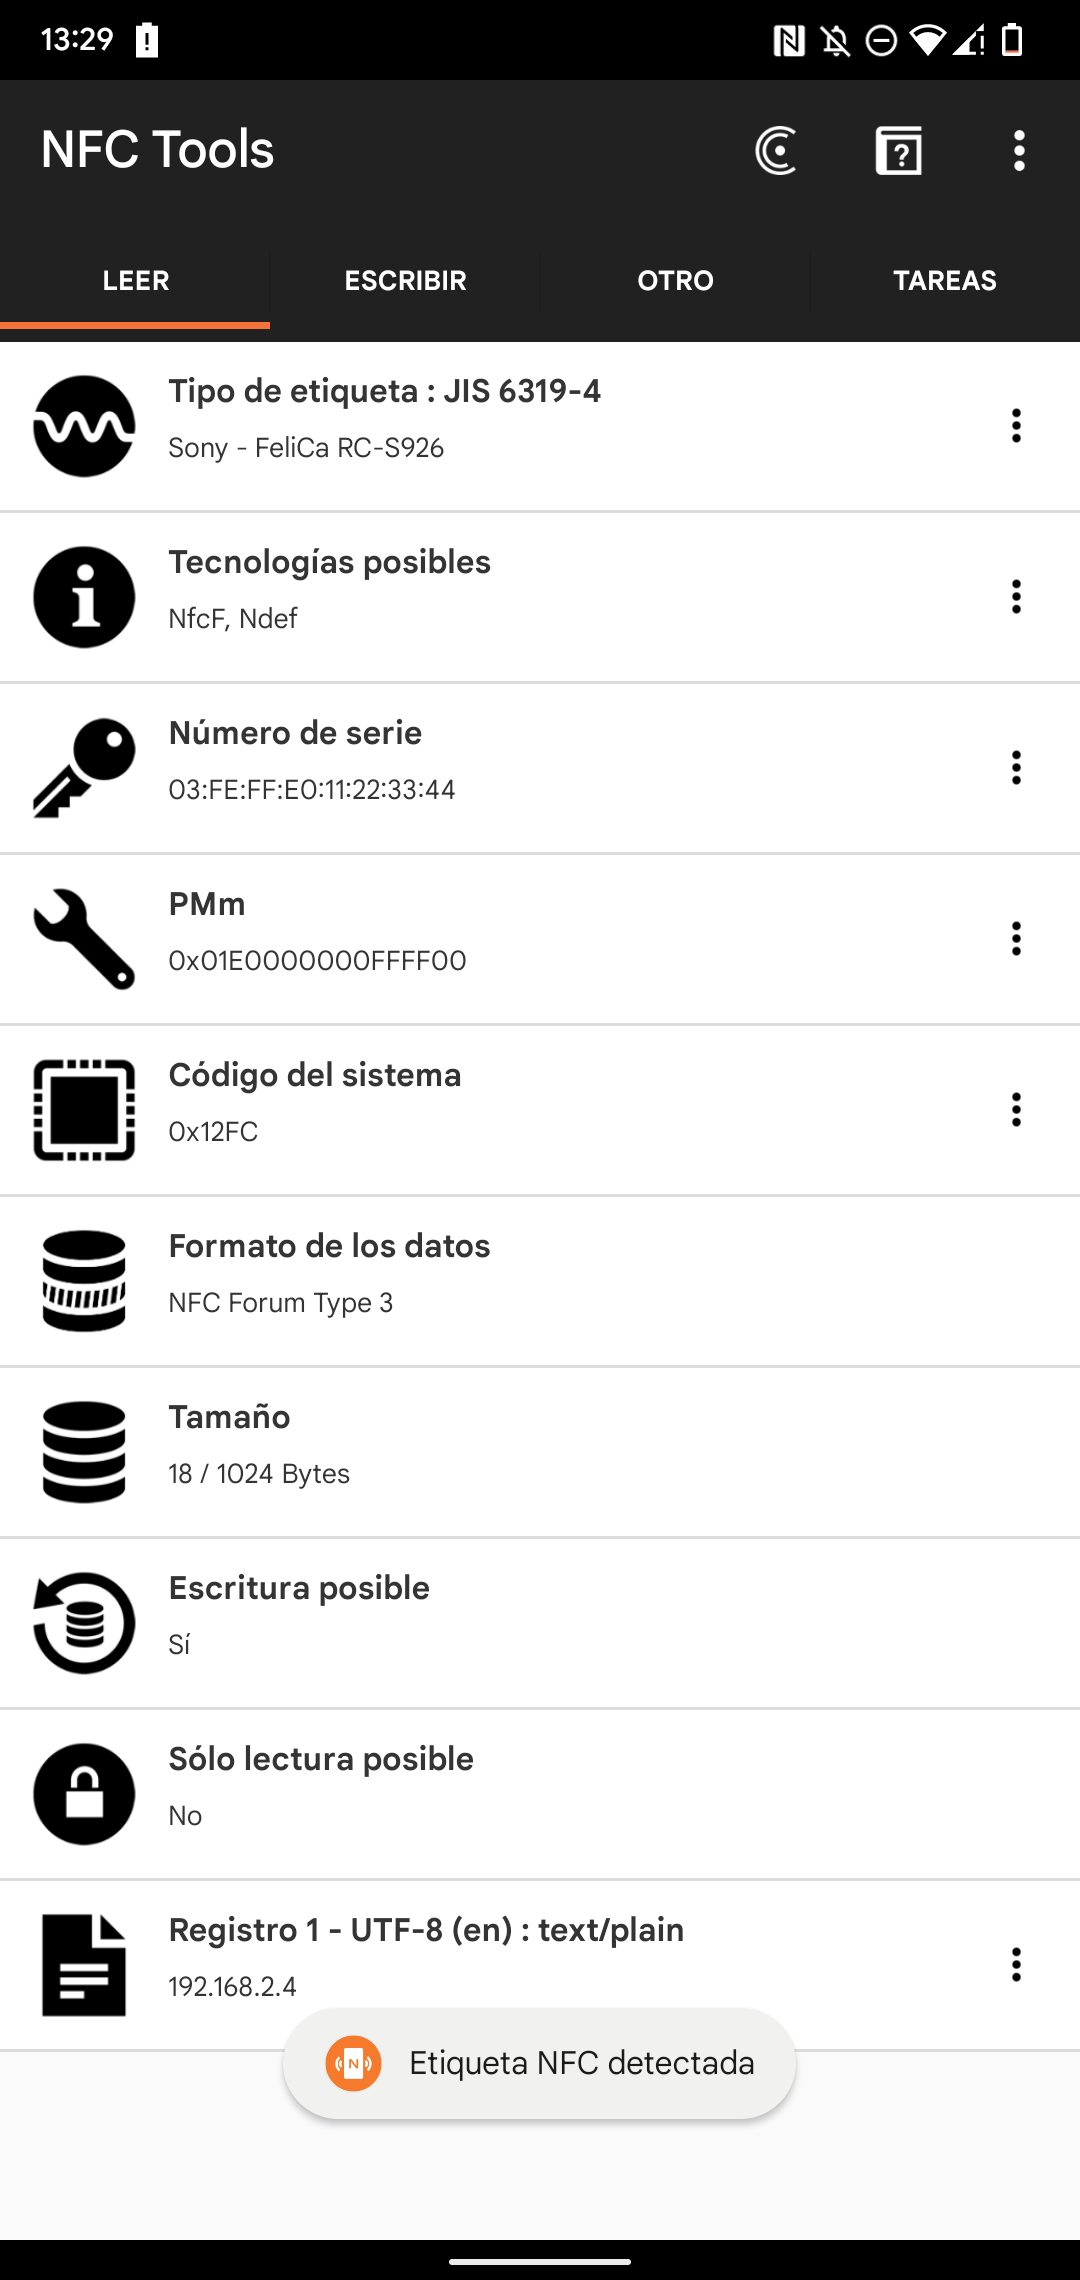
\includegraphics[width=0.3\textwidth]{fotos/lectura_raspberry.png}
    \caption{Lectura del módulo NFC de la Raspberry Pi con el fichero \emph{ndef} generado.}
\end{figure}

Con la creación de la tarjeta NFC con la IP de la Raspberry Pi hecha, ya solo
quedaba programar la lectura de la misma desde el móvil. Para ello, no hay más
que extraer el mensaje recibido del intent y ``traducir'' el mensaje, ya que
estos al enviarse se envían siguiendo la estructura de \emph{NDEF}. Para ello
hay que obtener la codificación del mensaje original así como el idioma,
información que viene dada en las propias cabeceras, y que de nuevo el libro de
O'Reilly \cite{ndef-explicado} se explica muy bien de forma gráfica:

\begin{figure}[H]
    \centering
    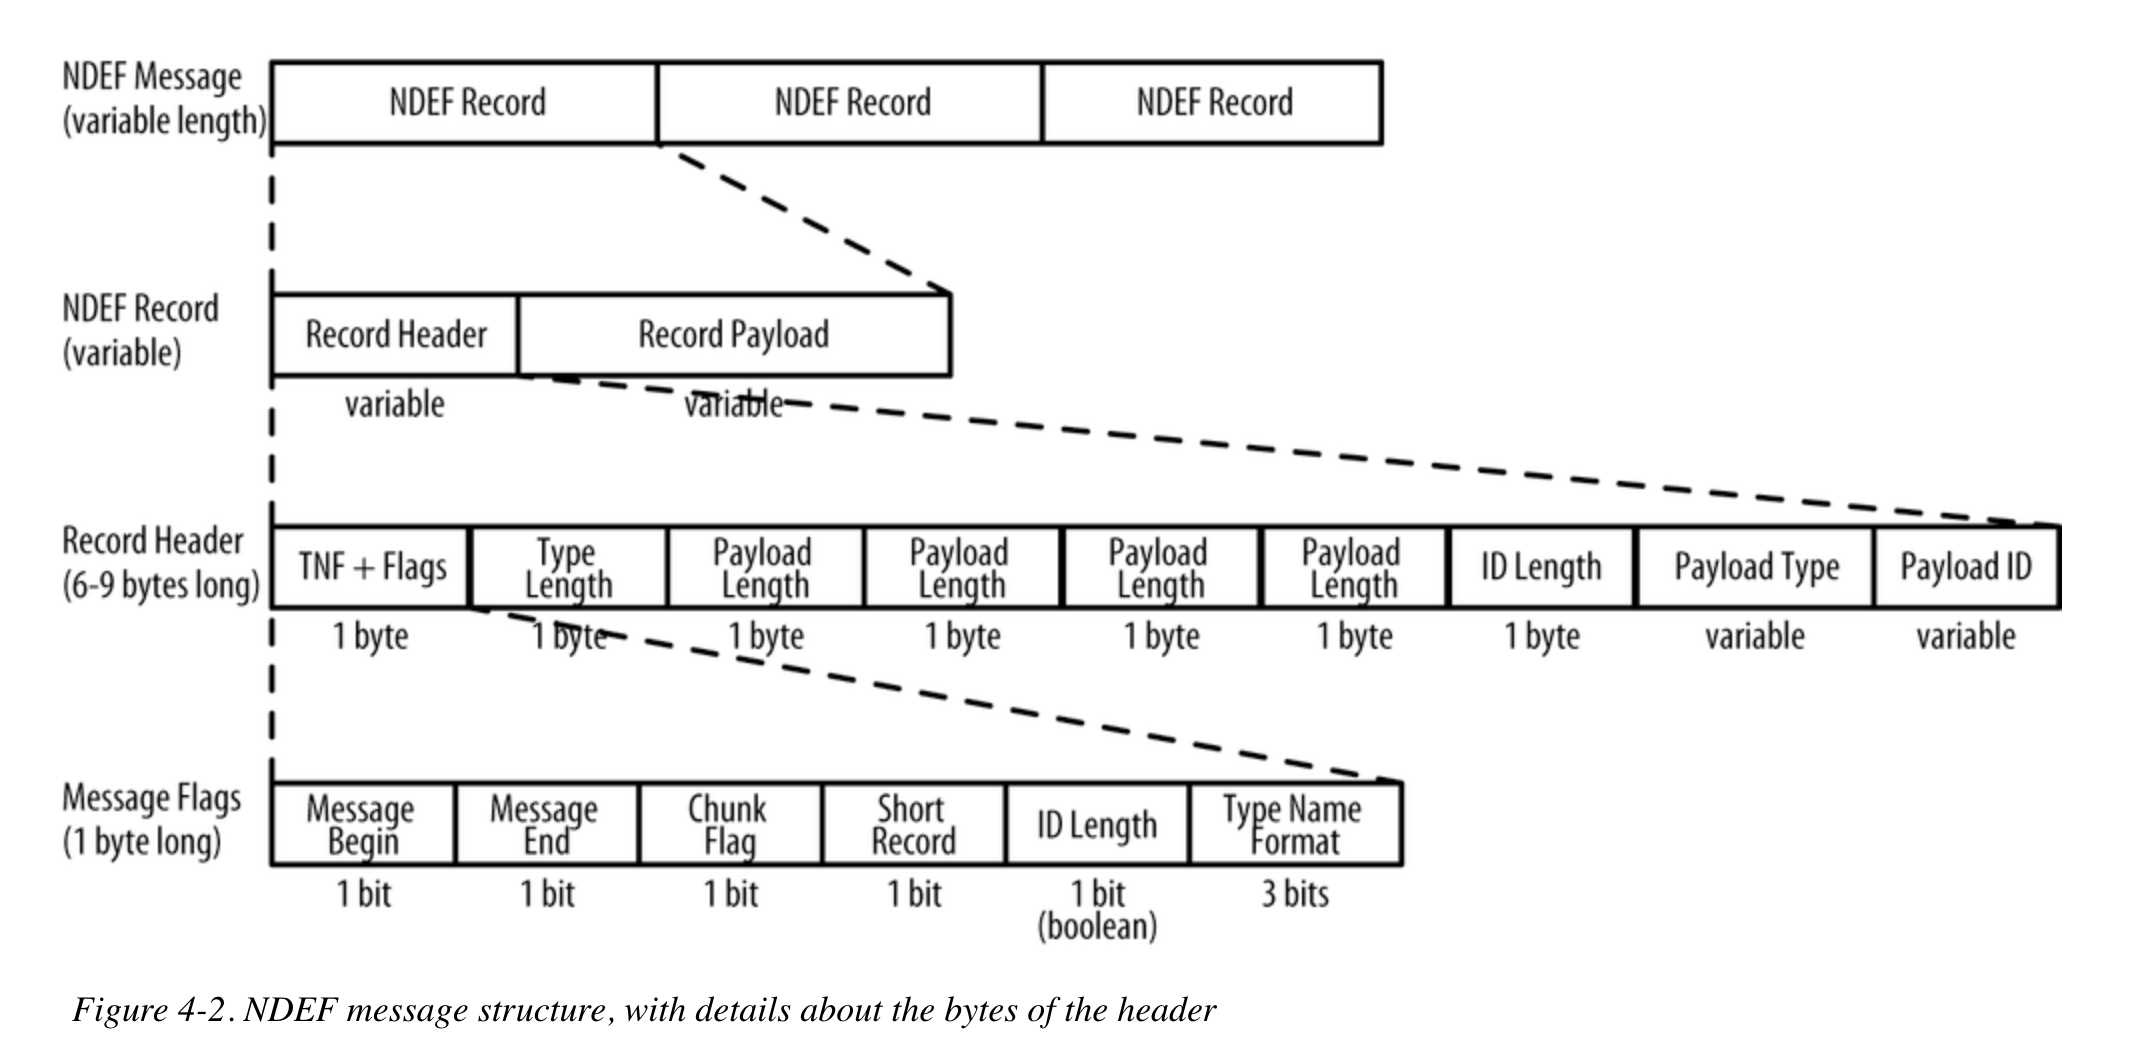
\includegraphics[width=0.7\textwidth]{fotos/estructura_ndef.png}
    \caption{Estructura interna de NDEF del libro de O’Reill \cite{ndef-explicado}.}
\end{figure}

De esta forma, y tras ser capaz de leer la IP del dispositivo receptor
correctamente, podemos dar por satisfecha esta necesidad, cumpliendo así el
``sub milestone'' de la comunicación NFC entre móvil y receptor.\\

Por lo que, en compañía del ya completado ``sub milestone'' anterior destinado a
la transmisión de audio, podemos dar por satisfecho de igual manera este PMV. 